\documentclass[twoside,11pt]{article}

% +
%  Name:
%     sc16.tex

%  Purpose:
%     Starlink Cookbook dealing with IFU data-product analysis (SC/16)

%  Authors:
%     AALLAN: Alasdair Allan (Starlink, University of Exeter)
%     MJC: Malcolm J. Currie (Starlink)

%  Copyright:
%     Copyright (C) 1997-2006 Particle Physics and Astronomy Research Council. Copyright (C) 1997-2005 Particle Physics and Astronomy Research Council.
%     Copyright (C) 2008 Science and Technology Facilities Council.
%     All Rights Reserved.
%
%  History:
%     01-SEP-2000 (AALLAN):
%        Original version.
%     24-NOV_2000 (AALLAN):
%        Added VIMOS information
%     30-DEC-2000 (AALLAN):
%        Cleanup for release
%     02-JAN-2001 (AALLAN):
%        Release version
%     2005 October 24 (MJC):
%        Update for revised DATACUBE and KAPPA.  Correct typographical
%        errors, spelling and punctuation.  Standardised the style.
%     2006 March 17 (MJC):
%        Velocity-map section now comprises an introduction, then two
%        paragraphs for the fitting and moments, the latter including
%        an illustration added now.  Include CLINPLOT in relevant
%        KAPPA visualisation tasks.  Mention COLLAPSE use for velocity
%        maps, and PERMAXES in the SPECDRE context.  Added remark that
%        DATACUBE is not limited to Wavelength.  Notified the existence
%        of getcurpos.csh in the C-shell scripts section. Further
%        spelling and typo's corrected.
%    2006 March 19 (MJC):
%        Add section on gridspec with illustrated example.
%    2006 June 16 (MJC):
%        Add CHANMAP, and smoothing of planes by BLOCK and GAUSMOOTH.
%        Introduce GAIA `3D' in a new illustrated subsection.  Enlarge
%        LateX graphics 25%.  Revise figure placement from default.
%    2008 July 4 (MJC):
%        Added section on locating features with CUPID and STILTS.
%        Update GAIA section and graphics; add new illustrated subsection
%        on three-dimensional rendering.  Mention PLUCK and PERMAXES.
%        Various minor updates.
%
%-

% ? Specify used packages
\usepackage{graphicx}        %  Use this one for final production.
% \usepackage[draft]{graphicx} %  Use this one for drafting.
% ? End of specify used packages

\pagestyle{myheadings}

% -----------------------------------------------------------------------------
% ? Document identification
% Fixed part
\newcommand{\stardoccategory}  {STARLINK Cookbook}
\newcommand{\stardocinitials}  {SC}
\newcommand{\stardocsource}    {sc\stardocnumber}

% Variable part - replace [xxx] as appropriate.
\newcommand{\stardocnumber}    {16.2}
\newcommand{\stardocauthors}   {A.~Allan \& Malcolm J. Currie}
\newcommand{\stardocdate}      {2008 July 4}
\newcommand{\stardocversion}   {Version 1.3}
\newcommand{\stardoctitle}     {The IFU Data-Product Cookbook}
\newcommand{\stardocmanual}    {}
\newcommand{\stardocabstract}
{This cookbook is a collection of material covering IFU data reduction and analysis. Along
with this material are pointers to more advanced documents dealing with the various packages,
and hints and tips about how to deal with commonly occurring problems.}

% ? End of document identification
% -----------------------------------------------------------------------------

% +
%  Name:
%     sc.tex
%
%  Purpose:
%     Template for Starlink Cookbook (SC) documents.
%     Refer to SUN/199
%
%  Authors:
%     AJC: A.J.Chipperfield (Starlink, RAL)
%     BLY: M.J.Bly (Starlink, RAL)
%
%  History:
%     16-JUN-1997 (BLY):
%        Original, based on SUN/SG templates.
%     {Add further history here}
%
% -

\newcommand{\stardocname}{\stardocinitials /\stardocnumber}
\markboth{\stardocname}{\stardocname}
\setlength{\textwidth}{160mm}
\setlength{\textheight}{230mm}
\setlength{\topmargin}{-2mm}
\setlength{\oddsidemargin}{0mm}
\setlength{\evensidemargin}{0mm}
\setlength{\parindent}{0mm}
\setlength{\parskip}{\medskipamount}
\setlength{\unitlength}{1mm}

% -----------------------------------------------------------------------------
%  Hypertext definitions.
%  ======================
%  These are used by the LaTeX2HTML translator in conjunction with star2html.

%  Comment.sty: version 2.0, 19 June 1992
%  Selectively in/exclude pieces of text.
%
%  Author
%    Victor Eijkhout                                      <eijkhout@cs.utk.edu>
%    Department of Computer Science
%    University Tennessee at Knoxville
%    104 Ayres Hall
%    Knoxville, TN 37996
%    USA

%  Do not remove the %begin{latexonly} and %end{latexonly} lines (used by
%  star2html to signify raw TeX that latex2html cannot process).
%begin{latexonly}
\makeatletter
\def\makeinnocent#1{\catcode`#1=12 }
\def\csarg#1#2{\expandafter#1\csname#2\endcsname}

\def\ThrowAwayComment#1{\begingroup
    \def\CurrentComment{#1}%
    \let\do\makeinnocent \dospecials
    \makeinnocent\^^L% and whatever other special cases
    \endlinechar`\^^M \catcode`\^^M=12 \xComment}
{\catcode`\^^M=12 \endlinechar=-1 %
 \gdef\xComment#1^^M{\def\test{#1}
      \csarg\ifx{PlainEnd\CurrentComment Test}\test
          \let\html@next\endgroup
      \else \csarg\ifx{LaLaEnd\CurrentComment Test}\test
            \edef\html@next{\endgroup\noexpand\end{\CurrentComment}}
      \else \let\html@next\xComment
      \fi \fi \html@next}
}
\makeatother

\def\includecomment
 #1{\expandafter\def\csname#1\endcsname{}%
    \expandafter\def\csname end#1\endcsname{}}
\def\excludecomment
 #1{\expandafter\def\csname#1\endcsname{\ThrowAwayComment{#1}}%
    {\escapechar=-1\relax
     \csarg\xdef{PlainEnd#1Test}{\string\\end#1}%
     \csarg\xdef{LaLaEnd#1Test}{\string\\end\string\{#1\string\}}%
    }}

%  Define environments that ignore their contents.
\excludecomment{comment}
\excludecomment{rawhtml}
\excludecomment{htmlonly}

%  Hypertext commands etc. This is a condensed version of the html.sty
%  file supplied with LaTeX2HTML by: Nikos Drakos <nikos@cbl.leeds.ac.uk> &
%  Jelle van Zeijl <jvzeijl@isou17.estec.esa.nl>. The LaTeX2HTML documentation
%  should be consulted about all commands (and the environments defined above)
%  except \xref and \xlabel which are Starlink specific.

\newcommand{\htmladdnormallinkfoot}[2]{#1\footnote{#2}}
\newcommand{\htmladdnormallink}[2]{#1}
\newcommand{\htmladdimg}[1]{}
\newenvironment{latexonly}{}{}
\newcommand{\hyperref}[4]{#2\ref{#4}#3}
\newcommand{\htmlref}[2]{#1}
\newcommand{\htmlimage}[1]{}
\newcommand{\htmladdtonavigation}[1]{}

% Define commands for HTML-only or LaTeX-only text.
\newcommand{\html}[1]{}
\newcommand{\latex}[1]{#1}

% Use latex2html 98.2.
\newcommand{\latexhtml}[2]{#1}

%  Starlink cross-references and labels.
\newcommand{\xref}[3]{#1}
\newcommand{\xlabel}[1]{}

%  LaTeX2HTML symbol.
\newcommand{\latextohtml}{{\bf LaTeX}{2}{\tt{HTML}}}

%  Define command to re-centre underscore for Latex and leave as normal
%  for HTML (severe problems with \_ in tabbing environments and \_\_
%  generally otherwise).
\newcommand{\setunderscore}{\renewcommand{\_}{{\tt\symbol{95}}}}
\latex{\setunderscore}

%  Redefine the \tableofcontents command. This procrastination is necessary
%  to stop the automatic creation of a second table of contents page
%  by latex2html.
\newcommand{\latexonlytoc}[0]{\tableofcontents}


% -----------------------------------------------------------------------------
%  Debugging.
%  =========
%  Remove % from the following to debug links in the HTML version using Latex.

% \newcommand{\hotlink}[2]{\fbox{\begin{tabular}[t]{@{}c@{}}#1\\\hline{\footnotesize #2}\end{tabular}}}
% \renewcommand{\htmladdnormallinkfoot}[2]{\hotlink{#1}{#2}}
% \renewcommand{\htmladdnormallink}[2]{\hotlink{#1}{#2}}
% \renewcommand{\hyperref}[4]{\hotlink{#1}{\S\ref{#4}}}
% \renewcommand{\htmlref}[2]{\hotlink{#1}{\S\ref{#2}}}
% \renewcommand{\xref}[3]{\hotlink{#1}{#2 -- #3}}
%end{latexonly}
% -----------------------------------------------------------------------------
% ? Document-specific \newcommand or \newenvironment commands.

% Figure environment. Defined for latex2html. #1 is postscript file
% #2 the qualifiers, #3 the gif file, #4 the label, #5 the caption.
\newcommand{\myfig} [5] {
  \begin{figure}[thb]
    \centering\includegraphics[#2]{#1}
    \typeout{#1 inserted on page \arabic{page}}
    \caption{\label{#4}#5}
  \end{figure}
  }
\begin{htmlonly}
  \newcommand{\myfig}[5]{
    \label{#4} \htmladdimg{#3}\\
    Figure: #5\\
    }
\end{htmlonly}

% ? End of document specific commands
% -----------------------------------------------------------------------------
%  Title Page.
%  ===========
\renewcommand{\thepage}{\roman{page}}
\begin{document}
\thispagestyle{empty}

%  Latex document header.
%  ======================
\begin{latexonly}
   CCLRC / {\sc Rutherford Appleton Laboratory} \hfill {\bf \stardocname}\\
   {\large Particle Physics \& Astronomy Research Council}\\
   {\large Starlink Project\\}
   {\large \stardoccategory\ \stardocnumber}
   \begin{flushright}
   \stardocauthors\\
   \stardocdate
   \end{flushright}
   \vspace{-4mm}
   \rule{\textwidth}{0.5mm}
   \vspace{5mm}
   \begin{center}
   {\Huge\bf  \stardoctitle \\ [2.5ex]}
   {\LARGE\bf \stardocversion \\ [4ex]}
   \end{center}
   \vspace{5mm}

% ? Add picture here if required for the LaTeX version.
%   e.g. \includegraphics[scale=0.3]{filename}
   \begin{center}
   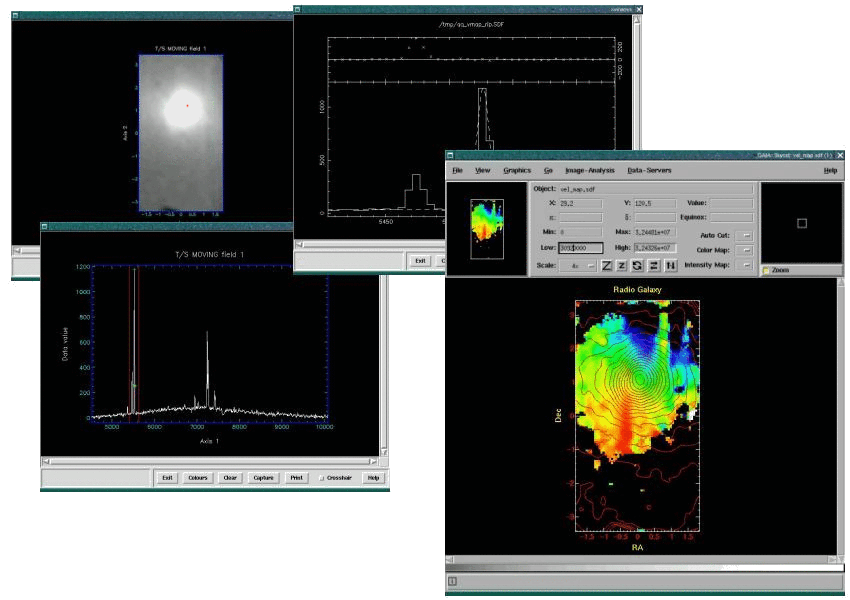
\includegraphics[scale=0.6]{sc16_cover}
   \end{center}
% ? End of picture

% ? Heading for abstract if used.
   \vspace{5mm}
   \begin{center}
      {\Large\bf Abstract}
   \end{center}
% ? End of heading for abstract.
\end{latexonly}

%  HTML documentation header.
%  ==========================
\begin{htmlonly}
   \xlabel{}
   \begin{rawhtml} <H1> \end{rawhtml}
      \stardoctitle\\
      \stardocversion\\
      \stardocmanual
   \begin{rawhtml} </H1> \end{rawhtml}

% ? Add picture here if required for the hypertext version.
%   e.g. \includegraphics[scale=0.7]{filename.ps}
   \htmladdimg{sc16_cover.png}

% ? End of picture

   \begin{rawhtml} <P> <I> \end{rawhtml}
   \stardoccategory\ \stardocnumber \\
   \stardocauthors \\
   \stardocdate
   \begin{rawhtml} </I> </P> <H3> \end{rawhtml}
      \htmladdnormallink{CCLRC}{http://www.cclrc.ac.uk} /
      \htmladdnormallink{Rutherford Appleton Laboratory}
                        {http://www.cclrc.ac.uk/ral} \\
      \htmladdnormallink{Particle Physics \& Astronomy Research Council}
                        {http://www.pparc.ac.uk} \\
   \begin{rawhtml} </H3> <H2> \end{rawhtml}
      \htmladdnormallink{Starlink Project}{http://www.starlink.ac.uk/}
   \begin{rawhtml} </H2> \end{rawhtml}
   \htmladdnormallink{\htmladdimg{source.gif} Retrieve hardcopy}
      {http://www.starlink.ac.uk/cgi-bin/hcserver?\stardocsource}\\

%  HTML document table of contents.
%  ================================
%  Add table of contents header and a navigation button to return to this
%  point in the document (this should always go before the abstract \section).
  \label{stardoccontents}
  \begin{rawhtml}
    <HR>
    <H2>Contents</H2>
  \end{rawhtml}
  \newcommand{\latexonlytoc}[0]{}
%  \htmladdtonavigation{\htmlref{\htmladdimg{sc16_cover.png}}
%        {stardoccontents}}

% ? New section for abstract if used.
  \section{\xlabel{abstract}Abstract}
% ? End of new section for abstract
\end{htmlonly}

% Shorthands for hypertext links.
% -------------------------------
\newcommand{\CCDPACK}{{\footnotesize CCDPACK}\normalsize}
\newcommand{\CCDPACKref}{\xref{\CCDPACK}{sun139}{}}
\newcommand{\CONVERT}{{\footnotesize CONVERT}\normalsize}
\newcommand{\CONVERTref}{\xref{\CONVERT}{sun55}{}}
\newcommand{\CUPID}{{\footnotesize CUPID}\normalsize}
\newcommand{\CUPIDref}{\xref{\CUPID}{sun237}{}}
\newcommand{\DATACUBE}{{\footnotesize DATACUBE}\normalsize}
\newcommand{\DATACUBEref}{\xref{\DATACUBE}{sun237}{}}
\newcommand{\FIGARO}{{\footnotesize FIGARO}\normalsize}
\newcommand{\FIGAROref}{\xref{\FIGARO}{sun86}{}}
\newcommand{\FITSref}{\htmladdnormallink{FITS}{http://fits.gsfc.nasa.gov/}}
\newcommand{\GAIA}{{\footnotesize GAIA}\normalsize}
\newcommand{\GAIAref}{\xref{\GAIA}{sun214}{}}
\newcommand{\IMSPEC}{{\footnotesize IMSPEC}\normalsize}
\newcommand{\IRAF}{\footnotesize{IRAF}\normalsize}
\newcommand{\IRAFref}{\htmladdnormallink{\IRAF}{http://iraf.noao.edu/iraf-homepage.html}}
\newcommand{\KAPPA}{{\footnotesize KAPPA}\normalsize}
\newcommand{\KAPPAref}{\xref{\KAPPA}{sun95}{}}
\newcommand{\PGPLOT}{{\footnotesize PGPLOT}\normalsize}
\newcommand{\PGPLOTref}{\htmladdnormallink{\PGPLOT}{http://astro.caltech.edu/\~{}tjp/pgplot/}}
\newcommand{\SPECDRE}{{\footnotesize SPECDRE}\normalsize}
\newcommand{\SPECDREref}{\xref{\SPECDRE}{sun86}{}}
\newcommand{\STILTS}{{\footnotesize STILTS}\normalsize}
\newcommand{\STILTSref}{\xref{\STILTS}{sun256}{}}

\newcommand{\ATV}{\footnotesize{ATV}\normalsize}
\newcommand{\CCDRED}{\footnotesize{CCDRED}\normalsize}
\newcommand{\FTOOLS}{\footnotesize{FTOOLS}\normalsize}
\newcommand{\HEASOFT}{\footnotesize{HEASOFT}\normalsize}
\newcommand{\INTEGRAL}{\footnotesize{INTEGRAL}\normalsize}
\newcommand{\ONEDSPEC}{\footnotesize{ONEDSPEC}\normalsize}
\newcommand{\SPECRED}{\footnotesize{SPECRED}\normalsize}
\newcommand{\XANADU}{\footnotesize{XANADU}\normalsize}
\newcommand{\XOASIS}{\footnotesize{XOASIS}\normalsize}

% arcminute symbol
\newcommand{\arcm}{\hbox{$^\prime$}}
%\begin{htmlonly}
%\renewcommand{\arcm}{'}}
%\end{htmlonly}

% arcsec symbol
\newcommand{\arcsec}{\arcm\hskip -0.1em\arcm}
%\begin{htmlonly}
%\renewcommand{\arcsec}{"}}
%\end{htmlonly}

% decimal-arcsecond symbol
\newcommand{\uarcs}{\hskip-0.27em\arcsec\hskip-0.02em}
\begin{htmlonly}
\newcommand{\uarcs}{"}}
\end{htmlonly}

% an environment for references (for the SST sstdiytopic command).
\newenvironment{refs}{\vspace{-4ex} % normally 3ex
                      \begin{list}{}{\setlength{\topsep}{0mm}
                                     \setlength{\partopsep}{0mm}
                                     \setlength{\itemsep}{0mm}
                                     \setlength{\parsep}{0mm}
                                     \setlength{\leftmargin}{1.5em}
                                     \setlength{\itemindent}{-\leftmargin}
                                     \setlength{\labelsep}{0mm}
                                     \setlength{\labelwidth}{0mm}}
                    }{\end{list}}



% -----------------------------------------------------------------------------
% ? Document Abstract. (if used)
%  ==================
\stardocabstract
% ? End of document abstract
% -----------------------------------------------------------------------------
% ? Latex document Table of Contents (if used).
%  ===========================================
 \newpage
 \vspace{3cm}

 \subsection*{Revision history}

 \begin{enumerate}
   \item 1st September 2000; Version 0.1 Original version (AA)
   \item 24th November 2000; Version 0.2 Added VIMOS information (AA)
   \item 12th December 2000; Version 0.3 Added IDL procedures (AA)
   \item 30th December 2000; Version 0.4 Cleanup for release (AA)
   \item 2nd January 2001; Version 1.0 Release version (AA)
   \item 30th September 2002; Version 1.0-1 Minor changes (AA)
   \item 2005 October; Version 1.1  Updated for DATACUBE version 1.1
                                    and major tidy. (MJC)
  \item 2006 March 17; Version 1.1-1 Add illustrated velmoment and gridspec
                       sections; mention CLINPLOT. (MJC)
  \item 2006 June 16; Version 1.1.-2 Introduce GAIA `3D' in a new
                      illustrated subsection.  List CHANMAP, and smoothing
                      of planes by BLOCK and GAUSMOOTH. (MJC)
  \item 2008 July 4;  Version 1.2  Add section on locating features with CUPID
                      and STILTS.  Update GAIA section and graphics; add new
                      illustrated subsection on three-dimensional rendering.
                      Mention PLUCK and PERMAXES.  (MJC)

 \end{enumerate}

 \vspace{10cm}
 \copyright \underline{1999--2008} Starlink, CCLRC, PPARC, STFC

 \begin{latexonly}
   \cleardoublepage
   \setlength{\parskip}{0mm}
   \latexonlytoc

   \newpage
   \listoffigures
   %\listoftables

   \setlength{\parskip}{\medskipamount}
   \markright{\stardocname}
 \end{latexonly}
% ? End of Latex document table of contents
% -----------------------------------------------------------------------------

\latex{\cleardoublepage}
\newpage
\renewcommand{\thepage}{\arabic{page}}
\setcounter{page}{1}

% The main text begins here.
% -----------------------------------------------------------------------------

\section{\xlabel{sc16_intro}Introduction\label{sc16_intro}}

Integral Field Spectroscopy (IFS) is a technique to produce a spectra
over a contiguous two-dimensional field, producing as a final data
product a three-dimensional data cube of the two spatial co-ordinate
axes plus an additional spectral axis, usually in wavelength.  Although
existing techniques, such as stepping a longslit spectrograph or
scanning a Fabry-Perot device, can produce such a data cube, the IFS
technique collects the data simultaneously with obvious savings in
observing efficiency.  However, IFS has only recently approached
maturity as a hardware technique.

The technique started with the use of lenslet arrays without fibres,
but the lack of a reformatting ability resulted in a short spectral
range.  The use of fibres improves on the lenslet-only technique, since
the field can be reformatted into a pseudo-slit which can be
dispersed by conventional spectrographs, and allows an IFS capability
to be retrofitted to existing spectrographs.  The earliest versions
used bare fibres (\emph{e.g.} INTEGRAL on WHT) but this suffers from
inefficient coupling to the telescope and incomplete field coverage
due to gaps between the fibre cores.  Both these problems can be solved
by coupling the fibres to micro-lenses.  Despite its greater technical
difficulty, this technique has been successfully prototyped, \emph{e.g.}\
SMIRFS on UKIRT and TEIFU on the WHT.  For infrared instruments working
in cryogenic or space environments which are hostile to fibres, the
technique of image slicing has been developed.  Here the field is
sliced into one-dimensional sections which are then reformatted into a
near-continuous long slit.

\section{\xlabel{sc16_datacubepackage}The Datacube Package\label{sc16_datacubepackage}}

The \htmladdnormallink{Starlink}{http://www.starlink.ac.uk/}
\DATACUBEref\ Package
\begin{latexonly}
(see SUN/237)
\end{latexonly}
of which this cookbook forms a part, mainly consists of C-shell ({\tt
csh}) scripts layered on top of various pieces of the Starlink
Software Collection (SSC).  This approach was a deliberate design
decision to allow the maximum amount of flexibility during data
visualisation.  Due to the relative lack of maturity in this still
developing field, it is difficult to say exactly what visualisation
tasks you may wish (or be required) to carry out to achieve the
underlying science.  While I (AA) have attempted to anticipate commonly
required tasks, the implementation of the package in easily
understandable, and modifiable, scripts allows you to make minor (or
even major) changes to the way they behave, although most of the
scripts already have \xref{command-line arguments}{sun237}{} which
can modify their behaviour to some extent\latex{ (see SUN/237 for
details)}.

It is to be hoped that enough ground work has been done so that the
approach to solving your data visualisation or manipulation problem is
obvious, even if \DATACUBE\ doesn't have a script or application to
exactly what you require.  I would welcome comments, contributions and
corrections to the package since I have been very much aware while
compiling it my on lack of experience in this fast evolving field, and
my own biases.  For instance, this document deals only briefly with
\IRAFref, while I am aware that there are \IRAF\ applications
available that will deal with spectral data cubes, my own lack of
familiarlity with the \IRAF\ package has lead to only spartan
coverage.  Comments should be sent to the Starlink support mailing
list
\htmladdnormallink{{\tt starlink@jiscmail.ac.uk} }{mailto:starlink@jiscmail.ac.uk}.

\section{\xlabel{sc16_reduction}Data reduction\label{sc16_reduction}}

Initial data reduction to remove instrumental effects such as flat
fielding and cosmic-ray removal, and mapping between the
two-dimensional detector co-ordinates and the data cube, is highly
instrument dependent.  The IFU instruments currently in use, with
obvious exceptions, tend not to be {\em common user} but instead {\em
fast-track} or {\em in-house} instruments.  This has had a strong
influence on the available data-reduction software.

\subsection{\xlabel{sc16_paradigms}Reduction paradigms\label{sc16_paradigms}}

There are two paradigms for IFS data reduction.  First, the
`traditional' method, adapted from multi-object spectroscopy (MOS),
where the output from each fibre is extracted by tracing the spectrum
and accounting for wavelength-dependent distortion (normally referred
to as the {\em MOS paradigm}).  More recently, with the arrival of
TEIFU where the fibre outputs are under-sampled by the detector, an
alternative paradigm has arisen (usually referred to as the {\em
longslit paradigm}).  Although the independence of the spatial samples
is lost due to the under-sampling of the point-spread function (PSF)
by the detector, it can be shown that this is irrelevant so long as
the target is critically sampled by the IFU; see Allington-Smith \&
Content (1998).  Here the methods adapted from MOS cannot be used and
the resulting dataset bears more resemblance to traditional longslit
spectroscopy than to MOS data.

\subsection{\xlabel{sc16_integral}INTEGRAL data\label{sc16_integral}}

\htmladdnormallink{INTEGRAL}{http://www.iac.es/proyect/integral/}
is an integral-field spectroscopic facility deployed at the Nasmyth
focus of the WHT, and channels the light into WYFFOS fibre
spectrograph.  Up to six fibre bundles are available, although only
three bundles are used in normal operation, with field sizes ranging
from 10 to 40 arcseconds and different fibre core sizes.  These
options allow observers to make the most efficient use of the
prevailing seeing conditions.\latex{ More information can be found
at {\tt http://www.iac.es/proyect/integral/}.}

Data-reduction facilities for the instrument are provided by the
\INTEGRAL\ \IRAFref\normalsize package which contains some standard tasks from
other \IRAF\ packages (such as \ONEDSPEC, \SPECRED, and \CCDRED) and
some custom tasks designed to deal with INTEGRAL data.  The package
can be
\htmladdnormallink{downloaded}{http://andromeda.roque.ing.iac.es/~astrosw/InstSoft/integral/integral-0.3.tar.gz}
from \goodbreak\latex{{\tt
http://andromeda.roque.ing.iac.es/$\sim$astrosw/InstSoft/integral/\-integral-0.3.tar.gz}}
\begin{htmlonly}
the IAC web pages
\end{htmlonly}
along with the package \htmladdnormallink{user
manual}{http://andromeda.roque.ing.iac.es/~astrosw/InstSoft/integral/manual_de_reducciones.ps.gz},
which contains installation instructions and a description of the
available reduction software\latex{ (see
Section~\ref{sc16_available})}.  It should be noted that to compile
the \INTEGRAL\ package requires the Starlink public-domain algorithms
(PDA) package to be present on your machine (see
\xref{SUN/194}{sun194}{}).

\subsection{\xlabel{sc16_oasis}OASIS data\label{sc16_oasis}}

\htmladdnormallink{OASIS}{http://www.cfht.hawaii.edu/Instruments/Spectroscopy/OASIS/}
is an integral field spectrograph for use with
\htmladdnormallink{AOB/PUEO}{http://www.cfht.hawaii.edu/Instruments/Imaging/AOB/}
although it can also be used at the direct f/8 Cassegrain focus as a
backup mode and for science programs necessitating IFS but with a
coarser spatial sampling defined by the natural seeing.  OASIS can
currently be used in two modes.  The imagery mode is used primary for
accurate pointing on objects.  Image quality has been optimized so that
high spatial resolution (0.$\uarcs$1) images can be obtained.  The
spectroscopic mode offers low-to-medium spectral resolution with a wide
range of spatial samplings performed by an array of hexagonal
micro-lenses.  Depending of the configuration employed, the
spectrographic field diameter varies from 1.5 arcsec to 10
arcsec.\latex{ More information can be found at {\tt
http://www.cfht.hawaii.edu/Instruments/Spectroscopy/OASIS/}.}

Data-reduction facilities is provided by the \htmladdnormallink{\XOASIS\
software}{http://www.cfht.hawaii.edu/Instruments/Spectroscopy/OASIS/Reduc/}
and detailed installation and `cookbook style' usage instructions
are available online.

\subsection{\xlabel{sc16_sauron}SAURON data\label{sc16_sauron}}

\htmladdnormallink{SAURON}{http://www.strw.leidenuniv.nl/sauron/}
is another IFS based on the TIGRE/\htmlref{OASIS}{sc16_oasis} concept
of a micro-lens array built for the WHT.  It has an array of 1500
square lens, and a wide field, either 10 or 35 arcsec$^2$.  Data
reduction is via pipeline software ({\footnotesize XSAURON\normalsize}
and {\footnotesize PALANTIR}\normalsize) especially developed for the
instrument which was modelled after the
\htmladdnormallink{\XOASIS}{http://www.cfht.hawaii.edu/Instruments/Spectroscopy/OASIS/Reduc/}
package.\latex{ More information about the instrument can be found
at {\tt http://www.strw.leidenuniv.nl/sauron/}.}

\subsection{\xlabel{sc16_gmos}GMOS data\label{sc16_gmos}}

The two Gemini Multi-Object Spectrographs
(\htmladdnormallink{GMOS}{http://www.gemini.edu/sciops/instruments/gmos/gmosIndex.html}),
one for each Gemini telescope, provides facilities for two-dimensional
spectroscopy over a contiguous field of $\sim$50 arcsec$^2$ with
0.2-arcsec sampling.  A small background field will be available at
fixed separation ($>1$ arcmin) from the main object field for accurate
background subtraction.  Details of the IFU itself can be found at
\htmladdnormallink{{\tt
http://www.gemini.edu/sciops/instruments/gmos/gmosIFU.html}}{http://www.gemini.edu/sciops/instruments/gmos/gmosIFU.html}.

\htmladdnormallink{Data-reduction
facilities}{http://www.gemini.edu/sciops/instruments/gmos/gmosDataRed.html}
for the instrument are provided in the Gemini \IRAFref\ package.

\subsection{\xlabel{sc16_cirpass}CIRPASS data\label{sc16_cirpass}}

\htmladdnormallink{CIRPASS}{http://www.ast.cam.ac.uk/~optics/cirpass/}
is a near-infrared spectrograph with a 499-element, lens and fibre,
integral-field unit to collect the light from the target object.
CIRPASS is available as a visitor instrument on the Gemini telescopes.
Users of CIRPASS are strongly encouraged to collaborate fully with the
instrument team in Cambridge to get the most out of their Gemini time.

The \htmladdnormallink{data-reduction and analysis software for
CIRPASS}{http://www.ast.cam.ac.uk/~optics/cirpass/docs/install_cirp_software.html}
runs under \IRAFref.  There is a
\htmladdnormallink{cookbook}{http://www.ast.cam.ac.uk/~optics/cirpass/datared/cookbook_sn1987a.php}
available\latex{ at
http://www.ast.cam.ac.uk/$\sim$optics/cirpass/datared/cookbook\_sn1987a.php}.


The final data product for the science data is an $x$,$y$,$\lambda$
\htmlref{data cube}{sc16_teifufile}\latex{ (see
Section~\ref{sc16_teifufile})}, which can be visualised as a
cube where the $z$-axis is wavelength and each plane is a picture of
what the IFU observed at that wavelength.

The first version of the \htmladdnormallink{data-reduction
package}{http://www.ast.cam.ac.uk/~optics/cirpass/docs/soft_spec.html}
will deal separately with the different types of data (\emph{e.g.}\
dome flats, sky flats, arc lamps, flux standards and target
observations).  For each type of data there are one or more pipeline
scripts to reduce the data, with each pipeline script running a series
of \IRAF\ tasks.

\latex{Links to more information on the ongoing development of the
reduction software can be found on the web at {\tt
http://www.ast.cam.ac.uk/$\sim$optics/cirpass/docs.html}.}

\subsection{\xlabel{sc16_smirfs}SMIRFS data\label{sc16_smirfs}}

\htmladdnormallink{SMIRFS}{http://star-www.dur.ac.uk/~jra/ukirt_ifu.html}
was constructed by the Durham group as a technology demonstrator for
the more ambitious integral-field units which Durham has producing and
continues to develop for the WHT and Gemini (\emph{e.g.}\
\htmlref{GMOS}{sc16_gmos}).  The IFU works with
\htmladdnormallink{CGS4}{http://www.jach.hawaii.edu/UKIRT/instruments/cgs4/cgs4.html}
on \htmladdnormallink{UKIRT}{http://www.jach.hawaii.edu/UKIRT/}
to provide IFS for the near infrared (1--2~$\mu$m in the $J$ and $H$
bands).  The SMIRFS IFU is available for use in collaboration with the
SMIRFS-IFU team, please contact \htmladdnormallink{Jeremy
Allington-Smith}{mailto:J.R.Allington-Smith@durham.ac.uk}\latex{
({\tt J.R.Allington-Smith@durham.ac.uk})}.

\latex{More information on the technical specifications of the
SMIRFS instrument, and the science that can be done with it, can be
found at {\tt http://star-www.dur.ac.uk/$\sim$jra/ukirt\_ifu.html}.}

\subsection{\xlabel{sc16_teifu}TEIFU data\label{sc16_teifu}}

\htmladdnormallink{TEIFU}{http://star-www.dur.ac.uk/~jra/teifu.html}
is a system for integral-field spectroscopy using
adaptively corrected images produced by the
\htmladdnormallink{ELECTRA}{http://www.cfai.dur.ac.uk/fix/adaptive-optics/area_main_ao.html}
and \htmladdnormallink{NAOMI}{http://www.ing.iac.es/Astronomy/instruments/naomi/} AO
systems on the WHT.  It is also able to operate in a stand-alone
mode without an adaptive-optics system.

Data-reduction facilities will be provided by the \IMSPEC\ \IRAF\
package which is under development at Durham.  No detailed information
is available at this time.

\subsection{\xlabel{sc16_uist}UIST data\label{sc16_uist}}

UIST is a general-purpose imager and spectrometer operating in the
1--5~$\mu$m range at
\htmladdnormallink{UKIRT}{http://www.jach.hawaii.edu/UKIRT/}, It was
commissioned in 2002 October, replacing all spectroscopy functions of
CGS4 except for echelle spectroscopy, all imaging functions of
IRCAM/TUFTI and all imaging functions of UFTI except the Fabry-Perot
filter.  It also includes a deployable image slicing IFU mounted in
the slit wheel.  Slicing mirrors are used to reformat a
$6.0\times3.3$-arcsec region of the sky into fourteen slices (the IFU
contains eighteen slicing mirrors but four are currently not usable),
each fifty pixels long, offset from one another along their length.  This
produces a staggered column on slitlets (as shown in
\begin{htmlonly}
the figure)
\end{htmlonly}
\latex{Figure~\ref{sc16_uist_fig})} which is used as the input for the
spectrometer in place of the long slit.

\myfig{sc16_uist}{height=0.6\textheight}{sc16_uist.png}{sc16_uist_fig}{The UIST staggered slitlets.}

Data acquisition, reduction and control software is provided by the
\htmladdnormallink{JAC}{http://www.jach.hawaii.edu/} ORAC system.  The
data-reduction part of the system,
\htmladdnormallink{ORAC-DR}{http://www.oracdr.org},
is provided by JAC and distributed by Starlink, and consists of a
fully automated perl-based \htmladdnormallink{pipelining
software}{http://monet.astro.uiuc.edu/adass98/Proceedings/economouf/}\latex{
(Economou\emph{et~al}. 1999)} sitting on top of the Starlink software
collection.  A general introduction to the ORAC-DR system can be found
in \xref{SUN/230}{sun230}{}.  The data-reduction recipes are
documented in \xref{SUN/246}{sun246}{} and at the
\htmladdnormallink{JAC web
site}{http://www.jach.hawaii.edu/UKIRT/instruments/uist/ifu/uistoracdr.html}.
An arc spectrum (Ar or Kr from the UIST calibration unit) is used to
straighten the staggered slitlets (which correspond to a wavelength
displacement from one slice to another) and apply a wavelength
calibration to the image.  The individual slice images will then be
copied to form $y$-$\lambda$ planes of an $x$,$y$,$\lambda$ data cube.
Recipes are also provided to carry out tasks such as flat-fielding and
flux-calibration.  Many of the recipes have specific requirements in
terms of, for instance, darks and flats fields which must be acquired
before a target observation is obtained and reduced on-line.


\subsection{\xlabel{sc16_vimos}VIMOS data\label{sc16_vimos}}

\htmladdnormallink{VIMOS}{http://www.eso.org/instruments/vimos/} has
been developed in fast track under ESO contract by the VIRMOS
consortium, headed by the Laboratoire d'Astrophysique de Marseille. In
IFU mode the field of view is between 13$\times$13 arcsec$^2$ and
54$\times$54 arcsec$^2$ at 0.33 or 0.67 arcsec fibre$^{-1}$.

Data-reduction software (DRS) will be made available by ESO, with the
procedures available as standalone packages, or under the VIMOS
pipeline-reduction software.\goodbreak
\htmladdnormallink{{\tt
http://www.oamp.fr/virmos/virmos\_publications.htm}}{http://www.oamp.fr/virmos/virmos_publications.htm}
contains links to various publications.  Two papers are scheduled for
the 2005 November {\em Astronomical Journal}.

\subsection{\xlabel{sc16_other}Other IFU instruments\label{sc16_other}}

Since the list of instruments was compiled for the original version of
this cookbook, many new Integral Field Units and area-spectroscopy
instruments have come online, such as
\htmladdnormallink{SINFONI}{http://www.eso.org/instruments/sinfoni/}
and \htmladdnormallink{FLAMES}{http://www.eso.org/instruments/flames/}
at the VLT,
\htmladdnormallink{GNIRS-IFU}{http://www.gemini.edu/sciops/instruments/nirs/nirsIndex.html}
at Gemini-S,
\htmladdnormallink{FISICA}{http://www.ctio.noao.edu/diroff/TALKS_PDF/Eikenberry_fisica_ctio05.pdf},
SNIFS; and several are being designed, for instance
\htmladdnormallink{KMOS-1}{http://www.cfai.dur.ac.uk/fix/projects/kmos1/kmos_main.html},
\htmladdnormallink{MUSE}{http://www.cfai.dur.ac.uk/fix/projects/muse/muse.html},
and FRIDA.

\newpage
\section{\xlabel{sc16_fileformat}File formats\label{sc16_fileformat}}

There are two main file format for IFS final data products, and one
further prospective format.  The \htmlref{first}{sc16_gmosfile} of
these file formats is a MOS style multi-extension
\FITSref\ file, and is
being put forward by the GEMINI group\latex{ (see
Section~\ref{sc16_gmosfile})}.  The other main format is an
$xy\lambda$---\htmlref{data cube}{sc16_teifufile} which is used by the
Durham group (\emph{i.e.}\ for SMIRFS and TEIFU data)\latex{ (see
Section~\ref{sc16_teifufile})}.

Of these two formats the more natural for data analysis is the TEIFU
style data cube, it has therefore been adopted as the standard format
by the major IFS groups in the UK, Durham (SMIRFS and TEIFU),
Cambridge (CIRPASS) and the ATC (UIST).
\htmlref{Conversion}{sc16_mef2cub} between the GMOS/CIRPASS MEF and UK
standard data cube formats\latex{ (see
Section~\ref{sc16_mef2cub})} will therefore need to be implemented
before these instruments are brought into general use.  The EOS VIMOS
instrument will provide its final data product in both MEF and
data-cube formats.

The final IFS format is still in draft, and is the new \IRAF\
spectroscopic \htmlref{file format}{sc16_iraf}\latex{
(see Section~\ref{sc16_iraf})}.  The specification is intended to
provide a general description for two-dimensional spectroscopic image
data, and should be able to represent long-slit, multi-object (MOS),
integral-field unit (IFU) and slitless spectroscopy.  Conversion
between this format and the standard data-cube format will be
implemented if the standard is adopted.

\subsection{\xlabel{sc16_gmosfile}The GMOS working format\label{sc16_gmosfile}}

Currently the final data product of the \htmlref{GMOS}{sc16_gmos} and
\htmlref{CIRPASS}{sc16_cirpass} data-reduction software is a
multi-extension \FITSref\ (MEF) file.  However, this format may be
replaced by the new \htmlref{\IRAF\ spectral
format}{sc16_iraf}\latex{ (see Section~\ref{sc16_iraf})} which is
currently in development by the IRAF group at NOAO.  The MEF is
similar to the standard NIRI format now used with GEMINI, and has a
binary FITS table with separate data, variance and quality planes.

\begin{table}[h]
\begin{center}
\begin{tabular}{cccccc}
No.\ & Type  & Name & Format & BITPIX & INH\\\hline
0  & ifs\_data.fits &  &                                     &  16 &   \\
1  & BINTABLE  & TAB & $16 \times${\em num.\,of fibres}      &   8 &   \\
2  & IMAGE     & SCI & $\lambda \times${\em num.\,of fibres} & $-$32 & F \\
3  & IMAGE     & VAR & $\lambda \times${\em num.\,of fibres} & $-$32 & F \\
4  & IMAGE     & DQ  & $\lambda \times${\em num.\,of fibres} &  16 & F \\ \hline
\end{tabular}
\caption{GEMINI MEF file format}
\end{center}
\protect\label{tab:mef_file}
\end{table}

The first extension is a binary FITS table with columns: ID, RA, DEC,
and SKY.  This table would hold information specific to individual
lenslets/fibres like relative fibre positions on the sky (RA, DEC),
whether the fibre is a sky or object spectrum (SKY), \emph{etc.}

The three image planes are like the \IRAF\
\htmladdnormallink{multispec
format}{http://iraf.noao.edu/iraf/docs/specwcs.ps.Z}; each row is a
separate spectrum.  This is a compact and efficient way of storing the
extracted spectra, avoiding having multiple extensions for each
individual spectra.  From \IRAF, \ONEDSPEC\ tasks like {\bf splot} can
be used on individual planes, and {\bf ldisplay} should be able to work
directly on the MEF.

\subsection{\xlabel{sc16_iraf}The {\em new} IRAF spectral format\label{sc16_iraf}}

A draft document has been written by the NOAO describing the new
\IRAFref\ \htmladdnormallink{spectroscopic file
format}{http://iraf.noao.edu/projects/ccdmosaic/imagedef/spec2d.html}.
This may, eventually, replace the GMOS \htmlref{working
format}{sc16_gmos} as the final science data product for
\htmlref{GMOS}{sc16_gmos} and \htmlref{CIRPASS}{sc16_cirpass}
observations.  An example header block is shown below for the CIRPASS
instrument.

\small\begin{verbatim}
OBJECT  = 'CIRPASS: m51 V 600s' / Observation title
OBJNAME = 'M 51    '           / Target object
OBJRA   = '13:29:24.00'        / Right ascension of object (hr)
OBJDEC  = '47:15:34.00'        / Declination of object (deg)
OBJEPOCH=               2000.1 / Epoch of object coordinates (yr)
EQUINOX =               2000.0 / Default coordinate equinox (yr)
RADECSYS= 'FK5     '           / Default coordinate system
RAUNIT  = 'hr      '           / Right ascension unit
DECUNIT = 'deg     '           / Declination unit
APERTURE= 'CIRPASS IFU'        / Aperture identification
APTYPE  = 'hexlens+fiber'      / Aperture type
APERDIA =                 0.36 / Aperture diameter (arcsec)
APERPA  =                 90.0 / Hexagon angle (deg)
APUNIT  = 'arcsec  '           / Aperture dimension unit
APPAUNIT= 'deg     '           / Aperture position angle unit
APEPOCH =               2000.1 / Aperture coordinate epoch (yr)
CRVAL1  =                  1.1 / Spectrum dispersion center (um)
CRVAL2  =                   0. / Spectrum cross-dispersion center (pixel)
CRPIX1  =               1024.0 / Spectrum center (pixel)
CRPIX2  =               1024.0 / Spectrum center (pixel)
CMIN1   =                  0.9 / Spectrum dispersion limit (um)
CMAX1   =                  1.3 / Spectrum dispersion limit (um)
CMIN2   =                 -1.5 / Spectrum cross-dispersion limit (pixel)
CMAX2   =                  1.5 / Spectrum cross-dispersion limit (pixel)
CTYPE1  = 'WAVE-WAV'           / Spectrum coordinate type
CTYPE2  = 'LINEAR  '           / Spectrum coordinate type
CUNIT1  = 'um'                 / Spectrum coordinate unit
CUNIT2  = 'pixel'              / Spectrum coordinate unit
CD1_1   =              0.00022 / Spec coord matrix (um/pixel)
CD1_2   =                  0.0 / Spec coord matrix (um/pixel)
CD2_1   =                  0.0 / Spec coord matrix (pixel/pixel)
CD2_2   =                  1.0 / Spec coord matrix (pixel/pixel)
SPECFWHM=                  2.0 / Fiber FWHM (pixel)
ARA0001 = '13:29:24.00'        / Aperture right ascension (hr)
ADEC0001= '47:15:34.00'        / Aperture declination (deg)
CRP20001=                500.0 / Spectrum center (pixel)
ARA0002 = '13:29:24.00'        / Aperture right ascension (hr)
ADEC0002= '47:15:34.36'        / Aperture declination (deg)
CRP20002=                504.0 / Spectrum center (pixel)
\end{verbatim}\normalsize

The aperture identification, {\tt APERTURE}, specifies the IFU.  The
aperture type {\tt APTYPE}, aperture diameter {\tt APERDIA}, and
aperture position angle {\tt APERPA} are the same for each spectrum.
This information can be used to \htmlref{construct a data
cube}{sc16_mef2cub}\latex{ (see Section~\ref{sc16_mef2cub})} or
spatial/dispersion displays in conjunction with the aperture centres.
The position angle is for one of the hexagonal edges and would orient
the hexagons (IFU lenslets) when reconstructing a spatial display or
data cube.  For a purely fibre IFU (such as SAURON) much the same
description would be used except the position angle would be
eliminated.

The centre of each spectrum in world co-ordinates is given by the {\tt
CRVAL} keywords.  In this example each spectrum is centred at about
1.1~$\mu$m in the dispersion direction ({\tt CRVAL1}) and zero pixels
in the cross-dispersion direction ({\tt CRVAL2}).  The cross-dispersion
co-ordinates are defined as pixels from the centre of the fibre
profile, since there is no real spatial information.  The region the
spectra cover in world co-ordinates are given by the {\tt CMIN} and
{\tt CMAX} keywords.  In this example the spectra cover the range 0.9
to 1.3~$\mu$m along the dispersion and $-$1.5 to 1.5 pixels relative to
the fibre profile centre.

The {\tt CD} keywords define the conversion between world co-ordinates
and pixels on the detector.  They also define any possible tilt of the
dispersion path relative to the detector pixels.  In this example the
dispersion is 0.22~nm per pixel along the first image axis (detector
rows) and there is no tilt.

The {\tt CRP} keywords override the {\tt CRPIX} keyword and provide
the positions of the fibre spectra on the detector.

The fibre full width at half maximum ({\tt SPECFWHM}) gives the fibre
profile FWHM at the detector in the units of the spatial WCS, in this
case pixels.  This is used to guide the tracing and extraction of
blended fibre profiles.

The {\tt ARA} and {\tt ADEC} keywords give the centre positions of
each lenslet element or fibre.  While it is desirable for the absolute
co-ordinates to be accurate it is more important that the relative
positions be fairly precise.  It is these keywords that determine the
reconstructed field and gives the IFU sampling pattern and
orientation.  The relative positions of the lenslets or fibres on the
sky is something that should be well-known for each IFU instrument.

\subsection{\xlabel{sc16_teifufile}The UK data-cube format\label{sc16_teifufile}}

The MOS-style \htmlref{MEF format}{sc16_gmosfile}, which is the end
product of the GMOS and CIRPASS data-reduction software, is not
particularly natural way of handling IFS data.  Indeed, under the
$longslit$ paradigm (used to reduce TEIFU data) these files cannot be
generated.  The TEIFU-style data cube format has therefore been
adopted as the standard UK IFS file format and will be used in the
analysis stages for both CIRPASS and UIST.  This adoption allows the
use of many of the generic applications within the SSC, which due to
the adoption of \xref{NDF}{sun33}{} as the standard file interchange
format for Starlink applications, has many tasks that can process
$N$-dimensional data.

A \htmlref{conversion program}{sc16_mef2cub} for GMOS and CIRPASS data
to a more easily analysed data cube, which will involve re-binning the
input spectra on to a rectangular array, is therefore
desirable\latex{ (see Section~\ref{sc16_mef2cub})}.

\begin{table}[h]
\begin{center}
\begin{tabular}{cccccl}
No.\ & Type  & Name & Format & BITPIX & Comment\\\hline
0 &ifs\_data.fits &  &          &       & \\
1 & IMAGE & SCI & $x \times y\times \lambda$ & $-$32 & 3-D science array \\
2 & IMAGE & VAR & $x \times y\times \lambda$ & $-$32 & 3-D variance array \\
3 & IMAGE & DQ  & $x \times y\times \lambda$ &    16 & 3-D data-quality array \\ \hline
\end{tabular}
\caption{TEIFU data-cube format}
\end{center}
\protect\label{tab:cub_file}
\end{table}

In the case of this format the IFU geometry information is no longer
needed, as the input spectra have already been rebinned, but it is
likely that (in the finalised file format) such information will be
included as a \FITSref\  binary table.

An example of the FITS header block from a TEIFU data cube is shown below.

\small\begin{verbatim}
SIMPLE  =                    T /  file does conform to FITS standard
BITPIX  =                   16 /  number of bits per data pixel
NAXIS   =                    3 /  number of data axes
NAXIS1  =                   59 /  length of data axis 1
NAXIS2  =                  110 /  length of data axis 2
NAXIS3  =                  961 /  length of data axis 3
EXTEND  =                    T /  FITS dataset may contain extensions
OBJECT  = 'T/S MOVING field  ' /  Title of the dataset
DATE    = '2000-10-05T17:50:52'/  file creation date (YYYY-MM-DDThh:mm:ss UTC)
BSCALE  =         3.126180E-02 /  True_value = BSCALE * FITS_value + BZERO
BZERO   =         6.089249E+02 /  True_value = BSCALE * FITS_value + BZERO
BLANK   =               -32768 /  Bad value
CD1_1   =               0.0625 / Axis rotation and scaling matrix
CD2_2   =               0.0625 / Axis rotation and scaling matrix
CD3_3   = 5.795317000000068219 / Axis rotation and scaling matrix
CRVAL1  =             -0.03125 / Axis 1 reference value
CRVAL2  =             -0.03125 / Axis 2 reference value
CRVAL3  = 7302.291864499999065 / Axis 3 reference value
CRPIX1  =                 29.5 / Axis 1 pixel value
CRPIX2  =                 55.0 / Axis 2 pixel value
CRPIX3  =                480.5 / Axis 3 pixel value
WCSDIM  =                    3
CTYPE1  = 'LINEAR  '           / Quantity represented by axis 1
CTYPE2  = 'LINEAR  '           / Quantity represented by axis 2
CTYPE3  = 'LAMBDA  '           / Quantity represented by axis 3
CD1_2   =                  0.0 / Axis rotation and scaling matrix
CD1_3   =                  0.0 / Axis rotation and scaling matrix
CD2_1   =                  0.0 / Axis rotation and scaling matrix
CD2_3   =                  0.0 / Axis rotation and scaling matrix
CD3_1   =                  0.0 / Axis rotation and scaling matrix
CD3_2   =                  0.0 / Axis rotation and scaling matrix
LTV3    =                -39.0
LTM1_1  =                  1.0
LTM2_2  =                  1.0
LTM3_3  =                  1.0
WAT0_001= 'system=image'
END
\end{verbatim}\normalsize

Here the the number and size of the cube dimensions is specified by
the {\tt NAXIS} keywords, and as with the \htmlref{\IRAF\ spectral
format}{sc16_iraf}\normalsize\ the {\tt CD} keywords define the conversion between
world co-ordinates and pixels on the detector, along with the tilt of
the dispersion path relative to the detector pixels.  While the {\tt
CRVAL} keywords defines the central value of each axis in world
co-ordinates, \emph{e.g.}\ in the case the spectral axis is centred on
$\sim$7302~\AA\ ({\tt CRVAL3}).

A full
\htmladdnormallink{dictionary}{http://iraf.noao.edu/projects/ccdmosaic/imagedef/fitsdic.html}
defining FITS header keywords which can be generated by the
data-acquisition system is provided on the web by the National Optical
Astronomy Observatories (NOAO)\latex{ at {\tt
http://iraf.noao.edu/projects/ccdmosaic/imagedef/fitsdic.html}}.

\subsection{\xlabel{sc16_mef2cub}MEF to data-cube format\label{sc16_mef2cub}}

In the Gemini \IRAF\ package the command {\bf gfcube} converts the
GMOS working format, which is currently being used as the science end
product file format for the GMOS and CIRPASS instruments, to a UK
standard $x$,$y$,$\lambda$ data cube in \FITSref\ format.

\subsection{\xlabel{sc16_converting}Format conversion\label{sc16_converting}}

The Starlink \CONVERTref\ package \latex{(see SUN/55)} can be used
to convert to and from the Starlink \xref{NDF}{sun33}{} format.
On-the-fly conversion of supported file formats (such as FITS and
\IRAF) can also be done by most Starlink applications if the \CONVERT\
package has been initialised.

\subsubsection{GMOS MEF to NDF}

The \CONVERTref\ package handles the GMOS/CIRPASS MEF
working format without complaint, as in the following example.

\begin{verbatim}
    % fits2ndf
    IN - Input FITS file(s) > gmos.fits
    1 file selected.
    OUT - Output NDF data structure(s) > out
    %
\end{verbatim}

Converting the MEF to a Starlink standard \xref{NDF}{sun33}{}, the
\FITSref\ binary table is converted into a normal NDF extension.  An
example of a resulting NDF is illustrated below.  The $<$~$>$ indicate
the data type of a component.  Those beginning with an underscore are
primitive types; others are structures.

\small\begin{verbatim}
IFS_FILE  <NDF>

   DATA_ARRAY     <ARRAY>
      ORIGIN(2)      <_INTEGER>
      DATA(2010,750)  <_REAL>

   MORE           <EXT>
      FITS_EXT_1      <TABLE>
         NROWS          <_INTEGER>
         COLUMNS        <COLUMNS>
            ID              <COLUMN>
               DATA(750)    <_INTEGER>

            RA          <COLUMN>
               COMMENT      <_CHAR*19>
               DATA(750)    <_REAL>

            DEC         <COLUMN>
               COMMENT      <_CHAR*19>
               DATA(750)    <_REAL>

            SKY         <COLUMN>
               COMMENT      <_CHAR*19>
               DATA(750)    <_INTEGER>

      FITS(790)       <_CHAR*80>

   VARIANCE       <ARRAY>
      DATA(2010,750)  <_REAL>
      ORIGIN(2)       <_INTEGER>

   QUALITY        <QUALITY>
      QUALITY         <ARRAY>
         DATA(2010,750)   <_UBYTE>
         ORIGIN(2)        <_INTEGER>
\end{verbatim}\normalsize

Here the right ascension and declination position of each fibre is preserved in the
{\tt FITS\_EXT\_1} NDF extension along with and array indicating
whether the fibre is `on sky'.

\subsubsection{TEIFU FITS to NDF}

The \CONVERTref\ package also handles the UK standard data
cube format (\emph{i.e.}\ TEIFU style data) without complaint, such as
in the example below.

\begin{verbatim}
    % fits2ndf
    IN - Input FITS file(s) > teifu.fits
    1 file selected.
    OUT - Output NDF data structure(s) > out
    %
\end{verbatim}

The \FITSref\ file is be converted it into a three-dimensional
\xref{NDF}{sun33}{} which, as \htmlref{discussed
earlier}{sc16_teifufile}\latex{ (see
Section~\ref{sc16_teifufile})} can be read by many existing
applications in the software collection.

\small\begin{verbatim}
IFS_FILE  <NDF>

   DATA_ARRAY     <ARRAY>
      ORIGIN(3)      <_INTEGER>
      DATA(59,110,961)  <_DOUBLE>
      BAD_PIXEL      <_LOGICAL>

   MORE           <EXT>
      FITS(45)       <_CHAR*80>

   TITLE          <_CHAR*18>
   WCS            <WCS>
      DATA(99)       <_CHAR*32>
\end{verbatim}\normalsize

\subsection{\xlabel{sc16_fits2ndf}GMOS vs.\ TEIFU format\label{sc16_fits2ndf}}

While both GMOS (MOS style) and TEIFU (data cube) representations of
IFS data are perfectly valid, there are several advantages to using the
data-cube format in preference to other options.  First, and perhaps
most importantly, for `longslit' paradigm instruments such as TEIFU
(and perhaps also CIRPASS) a MOS style data reduction is not possible
and therefore it is impossible to produce the first file type without
major problems.  Additionally a data-cube format is considered, by most
people, to be intrinsically easier to visualise.  Both these reasons
were taken under consideration when the data-cube format was adopted,
with consultation of Durham, Cambridge and the ATC, as the UK standard
format for this data.

\subsection{\xlabel{sc16_fitshdr}FITS header manipulation\label{sc16_fitshdr}}

Due to the still developing nature of the IFU file formats it is
possible that your data may have missing \FITSref\  header keywords, or
keywords which contain incorrect information.  If this is the case you
may need to manually edit your FITS file headers.

\subsubsection{Native FITS files}

A good package to use for \FITSref\ header (and data) manipulation is the
\htmladdnormallink{\FTOOLS}{
http://heasarc.gsfc.nasa.gov/docs/software/lheasoft/ftools/} software,
which is released along with
\htmladdnormallink{\XANADU}{http://heasarc.gsfc.nasa.gov/docs/software/lheasoft/xanadu/},
as part of the
\htmladdnormallink{\HEASOFT}{http://heasarc.gsfc.nasa.gov/docs/software/lheasoft/}
package from GSFC.\latex{ Further information about \HEASOFT, along
with detailed installation instructions, user manuals and a
development guide, can be found at {\tt
http://heasarc.gsfc.nasa.gov/docs/software/lheasoft/}.}

\subsubsection{The NDF FITS extension}

When a \FITSref\ file is converted to an \xref{NDF}{sun33}{} a FITS
extension---sometimes called the `airlock' to avoid confusion with
extensions within FITS files---is created.  This comprises a
one-dimensional array of character strings containing the imported
FITS header information.  On exporting a file from NDF format back to
FITS using \xref{{\bf ndf2fits}}{sun55}{NDF2FITS} the airlock contents
will be propagated back to the FITS file.  However, since the FITS
extension is not updated when an NDF is manipulated, any information
that can be derived directly from the NDF structure such as
dimensionality, units and axis information will replace any equivalent
information held in the FITS extension when it is exported.

The \KAPPAref\ package provides tools that allow you to read from, and
write to, an NDF FITS extension.  Example code using some of these
tools is shown later in this
\htmlref{document}{sc16_fitsheader}\latex{ (see
Section~\ref{sc16_fitsheader})}, and detailed documentation on these
tasks is available in \xref{SUN/95}{sun95}{se_fitsairlock}.

\subsection{\xlabel{sc16_fitsidl}FITS I/O with IDL\label{sc16_fitsidl}}

\htmladdnormallink{FITS
I/O}{http://idlastro.gsfc.nasa.gov/fitsio.html} with IDL can be
accomplished using the \htmladdnormallink{IDL Astronomy
Library}{http://idlastro.gsfc.nasa.gov/homepage.html} from the GSFC.
The IDL Astronomy Library contains four different sets of procedures
for reading, writing, and modifying \FITSref\ files.  The reason for having
four different methods of FITS I/O with IDL is partly historical, as
different groups developed the software independently.  However, each
method also has its own strengths and weakness for any particular
task.  For example, the procedure {\tt MRDFITS()}---which can read a
FITS table into an IDL structure---is the easiest procedure for
analyzing FITS files at the IDL prompt level (provided that one is
comfortable with IDL structures).  But mapping a table into an IDL
structure includes extra overhead, so that when performing FITS I/O at
the procedure level, it may be desirable to use more efficient
procedures such as {\tt FITS\_READ} and {\tt FTAB\_EXT}.

For example a data cube can be read into an IDL array using the {\tt
FXREAD} method.

\small\begin{verbatim}
      ; Read the FITS file
      fxread, 'ifu_file.fit', DATA, HEADER

      ; Determine the size of the image
      SIZEX=fxpar(header, 'NAXIS1')
      SIZEY=fxpar(header, 'NAXIS2')
      SIZEZ=fxpar(header, 'NAXIS3')

      ; Find the data type being read
      DTYPE=fxpar(header, 'BITPIX')
\end{verbatim}\normalsize

As can be seen, various values contained within the FITS header of the
original file can be obtained using the {\tt FXPAR} procedure.

Alternatively the {\tt MRDFITS} procedure can be used, as in this
example.

\small\begin{verbatim}
     ; Read the FITS file
     data = mrdfits('ifu_file.fit',0,header)
\end{verbatim}\normalsize

In both examples the image data is read into an IDL array called {\tt
DATA}, while the FITS header information is read into another array,
of TYPE {\tt STRING}, called {\tt HEADER}.

In addition FITS files can be read into IDL using the
\CONVERTref\normalsize\ package's \xref{on-the-fly file conversion}{sun55}{sect_auto}
ability\latex{ (see SUN/55 for more details)} and the \xref{{\tt
READ\_NDF}}{sun55}{READ_NDF} IDL function.

\subsection{\xlabel{sc16_ndfidl}NDF I/O with IDL\label{sc16_ndfidl}}

There are several methods for reading an \xref{NDF}{sun33}{} file into
IDL.  First the NDF can be converted to a FITS file using the
\xref{{\bf ndf2fits}}{sun55}{NDF2FITS} application in the \CONVERTref\
package,

\small\begin{verbatim}
    % ndf2fits comp=D
    IN - Input NDF data structure(s) /@section/ >
    1 NDF selected.
    OUT - Output FITS file(s) /@out/ > section.fit
    %
\end{verbatim}\normalsize

and then read into IDL using the \htmladdnormallink{IDL Astronomy
Library}{http://idlastro.gsfc.nasa.gov/homepage.html}\latex{ (as
in Section~\ref{sc16_fitsidl})}.  However, there are several other
approaches that can be taken.

The easiest approach is to use the \xref{{\tt
READ\_NDF}}{sun55}{READ_NDF} IDL procedure available with the
\CONVERT\ package.  When \CONVERT\ is installed, both the
IDL procedures {\tt READ\_NDF} and {\tt WRITE\_NDF} are placed in
{\tt \$CONVERT\_DIR} so, to make them available to IDL, that directory
must be added to the IDL search path.  This will be done if the
environment variable {\tt IDL\_PATH} has been set.

For example assuming we have a data cube called {\tt file.sdf} which is
of type {\tt \_REAL}

\small\begin{verbatim}
    IDL> data_array = read_ndf('file')
\end{verbatim}\normalsize

creates an IDL floating array, data\_array, with the same dimensions
as the NDF and containing the values from its {\tt DATA} component.

\small\begin{verbatim}
    IDL> data_array = read_ndf('file', !values.f_nan)
\end{verbatim}\normalsize

As above except that any occurrence of a bad value ({\tt VAL\_\_BADR}
as defined by the Starlink \xref{{\footnotesize
PRIMDAT}\normalsize}{sun39}{}\normalsize\ package) in the NDF will be replaced by
{\tt NaN} in the IDL array.

\small\begin{verbatim}
    IDL> var_array = read_ndf('file',comp='v')
\end{verbatim}\normalsize

creates an IDL byte array from the VARIANCE component of the same NDF.
Output of an IDL array is achieved using the corresponding \xref{{\tt
WRITE\_NDF}}{sun55}{WRITE_NDF} procedure, for example assuming {\tt
data\_array} is an IDL floating array then,

\small\begin{verbatim}
    IDL> write_ndf, data_array, 'file'
\end{verbatim}\normalsize

creates the NDF {\tt file.sdf} with the same dimensions as the IDL
array {\tt data\_array}, and writes the array to its DATA component
(of type {\tt \_REAL}).  No checks on bad values are made by default,
such checks can be carried out, \emph{e.g.}\

\small\begin{verbatim}
    IDL> write_ndf, data_array, 'file', !values.f_nan
\end{verbatim}\normalsize

Here any occurrence of the value {\tt NaN} in the array will be
replaced by the {\tt VAL\_\_BADR} value as defined by the Starlink
{\footnotesize PRIMDAT}\normalsize\ package.  While

\small\begin{verbatim}
    IDL> write_ndf, var_array, 'file', comp='v'
\end{verbatim}\normalsize

writes the IDL array {\tt var\_array} to the {\tt VARIANCE} component
of the NDF created above.  A check is made that the size of the array
corresponds with the size of the NDF.

There is yet another approach to read NDF data into IDL.  Again we
make use of the \CONVERT\ package, this time we use the \xref{{\bf
ndf2ascii}}{sun55}{NDF2ASCII} application to convert the NDF to a
ASCII text file so that we may use the IDL {\tt read\_ascii}
procedure, after generating an associated data template using the {\tt
ascii\_template} GUI.  For instance reading the file {\tt file.dat} in
the subdirectory {\tt ifu\_data}

\small\begin{verbatim}
    IDL> data_file = filepath('file.dat', SUBDIR='ifu_data')
    IDL> data_template = ascii_template(data_file)
    IDL> data = read_ascii(data_file, TEMPLATE=data_template)
\end{verbatim}\normalsize

we create an associated data template using {\tt ascii\_template} GUI
and read the data into the IDL structure {\tt data}.

We can similarly use the \xref{{\bf ndf2unf}}{sun55}{NDF2UNF}
application to create a sequential unformatted binary file and use the
{\tt read\_binary} and assocaited {\tt binary\_template} GUI to read
the data into IDL, \emph{e.g.}

\small\begin{verbatim}
    IDL> udata_file = filepath('binary.dat', SUBDIR='ifu_data')
    IDL> udata_template = binary_template(udata_file)
    IDL> udata = read_binary(udata_file, TEMPLATE=udata_template)
\end{verbatim}\normalsize

will return an IDL structure variable {\tt udata}.

The alternative more-low-level approach to reading either the ASCII or
binary unformated files can be taken, allowing you to bypass the
template GUIs.  More details can be found in \CONVERT\ documentation (see
\xref{SUN/55}{sun55}{}).

\newpage
\section{\xlabel{sc16_datacube}Data-cube manipulation\label{sc16_datacube}}

While the initial data-reduction software for IFUs is highly
instrument dependent, the data analysis of the final science data
product for all these instruments should be fairly generic.  The end
product of the data reduction for IFS is, almost naturally, an
$x$,$y$,$\lambda$ data cube.  For instruments not working in the
optical and infrared regimes, the third axis may also be in some other
spectral co-ordinate system, such as frequency.  Once assembled, with
associated variance and quality arrays, scientifically interesting
information can be extracted from the cube.

\subsection{\xlabel{sc16_exist}Existing software\label{sc16_exist}}

For {\em long-slit paradigm} instruments a data cube is the only data
product available, as overlapping point-spread functions mean that the
spectral data must be resampled.  For {\em MOS paradigm} data, while
the individual spectra are available, data visualisation is often
intrinisically more intuitive if done on resampled data cubes.  As
such, this cookbook will (in the main) only deal with applications
that handle the data-cube format.  If you have already sourced the
Starlink {\tt /star/etc/login} and {\tt /star/etc/cshrc}
files{\footnote {\tt /star/etc/ is for a standard Starlink installation,
but the Starlink software may be in a different directory tree on your
system.} then the commands {\tt kappa}, {\tt figaro}, and {\tt
ccdpack} will set up access to the \KAPPAref, \FIGAROref, and
\CCDPACKref\ tasks respectively, including most of the following
applications.

\subsubsection{Arithmetic Operations}

Some of the most fundamental operations you might wish to perform on a
data cube are the arithmetic operations of addition, subtraction,
multiplication and division, both by scalars and other data cubes.  All
these basic operations, and additional more complicated ones, can be
carried out using tasks from the \KAPPAref\ package.
\latex{Detailed documentation for all of these tasks can be found
in SUN/95.}

\begin{itemize}

\item{\xref{{\bf add}}{sun95}{ADD}}\\
Adds two NDF data structures
\item{\xref{{\bf cadd}}{sun95}{CADD}}\\
Adds a scalar to an NDF data structure
\item{\xref{{\bf calc}}{sun95}{CALC}}\\
Evaluates a mathematical expression
\item{\xref{{\bf cdiv}}{sun95}{CDIV}}\\
Divides an NDF by a scalar
\item{\xref{{\bf cmult}}{sun95}{CMULT}}\\
Multiplies an NDF by a scalar
\item{\xref{{\bf csub}}{sun95}{CSUB}}\\
Subtracts a scalar from an NDF data structure
\item{\xref{{\bf div}}{sun95}{DIV}}\\
Divides one NDF data structure by another
\item{\xref{{\bf maths}}{sun95}{MATHS}}\\
Evaluates mathematical expressions applied to NDF data structures
\item{\xref{{\bf mult}}{sun95}{MULT}}\\
Multiplies two NDF data structures
\item{\xref{{\bf normalize}}{sun95}{NORMALIZE}}\\
Normalises one NDF to a similar NDF by calculating a scale factor and zero-point difference
\item{\xref{{\bf pow}}{sun95}{POW}}\\
Takes the specified power of each pixel of a data array
\item{\xref{{\bf rift}}{sun95}{RIFT}}\\
Adds a scalar to a section of an NDF data structure to correct rift-valley defects
\item{\xref{{\bf sub}}{sun95}{SUB}}\\
Subtracts one NDF data structure from another
\item{\xref{{\bf thresh}}{sun95}{THRESH}}\\
Edits an NDF such that array values below and above two thresholds take constant values
\end{itemize}

\subsubsection{Cube manipulation}

Slightly more complex is manipulation and resampling of the data cube
itself.  The most important utilities available to do this within
\KAPPA\ are the \xref{{\bf collapse}}{sun95}{COLLAPSE},
\xref{{\bf chanmap}}{sun95}{CHANMAP}, \xref{{\bf ndfcopy}}{sun95}{NDFCOPY},
and \xref{{\bf pluck}}{sun95}{PLUCK} applications.  {\bf collapse} can
produce \htmlref{white-light and passband}{sc16_vis} images\latex{ (see
Section~\ref{sc16_vis})} and velocity maps by the appropriate
selection of statistic.  {\bf chanmap} creates a grid of passbands.
{\bf ndfcopy} can extract a single spectrum (along pixel axes) or
\htmlref{arbitrary cube sections}{sc16_vis} \latex{ (again see
Section~\ref{sc16_vis} for details)}, while {\bf pluck} uses
interpolation to extract at {\em arbitrary} positions, such as a
spectrum at nominated equatorial co-ordinates, or an image at a given
wavelength or frequency.  Some applications require the spectral
axis to be the first or the third axis; {\bf permaxes} allows
shuffling of the pixel axes.

\begin{itemize}
\item{\xref{{\bf chanmap}}{sun95}{CHANMAP}}\\
Creates a channel map from a cube NDF by compressing slices along a nominated axis
\item{\xref{{\bf collapse}}{sun95}{COLLAPSE}}\\
Reduces the number of axes in an $N$-dimensional NDF by compressing it along a nominated axis
\item{\xref{{\bf compadd}}{sun95}{COMPADD}}\\
Reduces the size of an NDF by adding values in rectangular boxes
\item{\xref{{\bf compave}}{sun95}{COMPAVE}}\\
Reduces the size of an NDF by averaging values in rectangular boxes
\item{\xref{{\bf compick}}{sun95}{COMPICK}}\\
Reduces the size of an NDF by picking equally spaced pixels
\item{\xref{{\bf flip}}{sun95}{FLIP}}\\
Reverses an NDF's pixels along a specified dimension
\item{\xref{{\bf ndfcopy}}{sun95}{NDFCOPY}}\\
Copies an NDF, or an NDF section, to a new location
\item{\xref{{\bf permaxes}}{sun95}{PERMAXES}}\\
Permutes an NDF's pixel axes
\item{\xref{{\bf pixdupe}}{sun95}{PIXDUPE}}\\
Expands an NDF by pixel duplication
\item{\xref{{\bf pluck}}{sun95}{PLUCK}}\\
Plucks slices from an NDF at arbitrary positions
\item{\xref{{\bf regrid}}{sun95}{REGRID}}\\
Applies a geometrical transformation to an NDF
\item{\xref{{\bf segment}}{sun95}{SEGMENT}}\\
Copies polygonal segments from one NDF into another
\item{\xref{{\bf slide}}{sun95}{SLIDE}}\\
Realigns an NDF using a translation.
\end{itemize}

\subsubsection{Two-dimensional manipulation}

While IFU data is intrinsically three dimensional there are times when
it is necessary to deal with two dimensional images during analysis
(\emph{e.g.}\ velocity maps).  Some potentially useful \KAPPA\
applications which are restricted to handling two-dimensional files
are

\begin{itemize}
\item{\xref{{\bf look}}{sun95}{LOOK}}\\
Outputs the values of a sub-array of a two-dimensional data array to the screen or a text file
\item{\xref{{\bf median}}{sun95}{MEDIAN}}\\
Smooths a two-dimensional data array using a weighted median filter
\end{itemize}

Some tasks operate in two dimensions, but apply processing to a series
of planes in a cube.  They permit, for example, to smooth spatially
while retaining the spectral resolution.

\begin{itemize}
\item{\xref{{\bf block}}{sun95}{BLOCK}}\\
Smooths an NDF using a one- or two-dimensional square or rectangular box filter
\item{\xref{{\bf gausmooth}}{sun95}{GAUSMOOTH}}\\
Smooths a one- or two-dimensional NDF using a Gaussian filter
\item{\xref{{\bf rotate}}{sun95}{ROTATE}}\\
Rotates two-dimensional NDF about its centre through any angle
\end{itemize}


\subsubsection{Pixel Operations}

There are several applications which can carry out operations on
individual pixels, the most general of these is \xref{{\bf
chpix}}{sun95}{CHPIX} which can replace the pixel value of a single,
or region, of pixels with an user defined value (including the bad
\xref{magic value}{sun95}{se_masking}).

\begin{itemize}
\item{\xref{{\bf chpix}}{sun95}{CHPIX}}\\
Replaces the values of selected pixels in an NDF
\item{\xref{{\bf errclip}}{sun95}{ERRCLIP}}\\
Removes pixels with large errors from an NDF
\item{\xref{{\bf fillbad}}{sun95}{FILLBAD}}\\
Removes regions of bad values from an NDF
\item{\xref{{\bf nomagic}}{sun95}{NOMAGIC}}\\
Replaces all occurrences of \xref{magic value}{sun95}{se_masking}\latex{(see SUN/95 for details)}
pixels in an NDF array with a new value
\item{\xref{{\bf numb}}{sun95}{NUMB}}\\
Counts the number of elements of an NDF with values or absolute values above or below a threshold
\item{\xref{{\bf substitute}}{sun95}{SUBSTITUTE}}\\
Replaces all occurrences of a given value in an NDF array with another value
\end{itemize}

\subsubsection{Other tools and file manipulation}

Building processing scripts from the Starlink applications can involve
you manipulating or querying information about structures within the
NDF file itself, three useful \KAPPAref\ commands to do this are listed
below.

\begin{itemize}
\item{\xref{{\bf ndftrace}}{sun95}{NDFTRACE}}\\
Displays the attributes of an NDF data structure
\item{\xref{{\bf parget}}{sun95}{PARGET}}\\
Obtains the value or values of an application parameter
\item{\xref{{\bf stats}}{sun95}{STATS}}\\
Computes simple statistics for an NDF's pixels
\end{itemize}

In some cases NDF information must be modified after a processing step
(\emph{e.g.}\ the NDF title) or, in the case of a \htmlref{newly
created}{sc16_newndf} NDF\latex{ (see Section~\ref{sc16_newndf})},
we must generate inital values.  \KAPPA\ provides various tools to
manipulate NDF extensions.

\begin{itemize}
\item{\xref{{\bf axlabel}}{sun95}{AXLABEL}}\\
Sets a new label value for an axis within an NDF data structure
\item{\xref{{\bf axunits}}{sun95}{AXUNITS}}\\
Sets a new units value for an axis within an NDF data structure
\item{\xref{{\bf setaxis}}{sun95}{SETAXIS}}\\
Sets values for an axis array component within an NDF data structure
\item{\xref{{\bf setbad}}{sun95}{SETBAD}}\\
Sets new bad-pixel flag values for an NDF
\item{\xref{{\bf setbb}}{sun95}{SETBB}}\\
Sets a new value for the quality bad-bits mask of an NDF
\item{\xref{{\bf setbound}}{sun95}{SETBOUND}}\\
Sets new bounds for an NDF
\item{\xref{{\bf setext}}{sun95}{SETEXT}}\\
Manipulates the contents of a specified NDF extension
\item{\xref{{\bf setlabel}}{sun95}{SETLABEL}}\\
Sets a new label for an NDF data structure
\item{\xref{{\bf setmagic}}{sun95}{SETMAGIC}}\\
Replaces all occurrences of a given value in an NDF array with the bad value
\item{\xref{{\bf setnorm}}{sun95}{SETNORM}}\\
Sets a new value for one or all of an NDF's axis-normalisation flags
\item{\xref{{\bf setorigin}}{sun95}{SETORIGIN}}\\
Sets a new pixel origin for an NDF
\item{\xref{{\bf settitle}}{sun95}{SETTITLE}}\\
Sets a new title for an NDF data structure
\item{\xref{{\bf settype}}{sun95}{SETTYPE}}\\
Sets a new numeric type for the data and variance components of an NDF
\item{\xref{{\bf setunits}}{sun95}{SETUNITS}}\\
Sets a new units value for an NDF data structure
\item{\xref{{\bf setvar}}{sun95}{SETVAR}}\\
Sets new values for the variance component of an NDF data structure
\end{itemize}

\subsubsection{Visualisation}

Combined with the \htmlref{graphics devices commands}{sc16_graphics}\latex{ (see
Section~\ref{sc16_graphics})} the following applications, especially
{\bf clinplot}, {\bf display}, {\bf linplot} and {\bf contour} act as the backbone
for image display, and some complex effects can be generated using
these elemental tasks.

\begin{itemize}
\item{\xref{{\bf clinplot}}{sun95}{CLINPLOT}}\\
Draws a spatial grid of line plots for an axis of a cube NDF
\item{\xref{{\bf contour}}{sun95}{CONTOUR}}\\
Contours a two-dimensional NDF
\item{\xref{{\bf cursor}}{sun95}{CURSOR}}\\
Reports the co-ordinates of positions selected using the cursor
\item{\xref{{\bf display}}{sun95}{DISPLAY}}\\
Displays a one- or two-dimensional NDF
\item{\xref{{\bf drawsig}}{sun95}{DRAWSIG}}\\
Draws +/-n standard-deviation lines on a line plot
\item{\xref{{\bf linplot}}{sun95}{LINPLOT}}\\
Draws a line plot of the data values in a one-dimensional NDF
\item{\xref{{\bf profile}}{sun95}{PROFILE}}\\
Creates a one-dimensional profile through an $N$-dimensional NDF
\end{itemize}

\subsubsection{Mosaics}

Mosaicking multiple IFU data cubes together is something you may well
wish to consider, unfortuantely there are \htmlref{problems}{sc16_mos}
involved in doing so\latex{ (see Section~\ref{sc16_mos})}, however,
the following tasks from \KAPPA\ may be useful

\begin{itemize}
\item{\xref{{\bf wcsalign}}{sun95}{WCSALIGN}}\\
Aligns a group of NDFs using World Co-ordinate System information
\item{\xref{{\bf wcsmosaic}}{sun95}{WCSMOSAIC}}\\
Tiles a group of NDFs using World Co-ordinate System information
\end{itemize}

along with the following tasks from \CCDPACKref.

\begin{itemize}
\item{\xref{{\bf makemos}}{sun139}{MAKEMOS}}\\
Makes a mosaic by combining and (optionally) normalising a set of images
\item{\xref{{\bf drizzle}}{sun139}{DRIZZLE}}\\
Resamples and mosaics using the drizzling algorithm
\end{itemize}

\subsubsection{Spectral fitting\label{spectral_fitting}}

Some of the most useful applications available for spectral fitting
and manipulation live inside \FIGAROref\ as part of \SPECDREref.  Some
of these applications work on individual spectra, however, others read
a whole cube at once and work on each row in turn.  A possible problem
at this stage is that many of these applications expect the
spectroscopic axis to be the first in the cube, whereas for the
current generation of IFU data cubes the spectral axis is typically the
third axis in the cube.  \KAPPA\ \xref{{\bf permaxes}}{sun95}{PERMAXES}
can reconfigure the cube as needed by the various packages.   A full
list of \xref{\SPECDRE\ applications}{sun86}{classifspecdre} can be
found in SUN/86.

One of the fundamental building blocks of spectral analysis is
gaussian fitting, amougst other tools, \FIGARO\ provides the
\xref{{\bf fitgauss}}{sun86}{FITGAUSS} application (part of \SPECDRE)
to carry out this task.

FITGAUSS is especially well suited to automation inside a script.
For example,

\small\begin{verbatim}
      fitgauss \
         in=${spectrum} mask1=${low_mask} mask2=${upp_mask} \
         cont=${cont} peak=${peak} fwhm=${fwhm} reguess=no remask=no \
         ncomp=1 cf=0 pf=0 wf=0 comp=${component} fitgood=yes \
         centre=${position} logfil=${fitfile} device=xwin \
         dialog=f
\end{verbatim}\normalsize

we call the {\bf fitgauss} routine here specifying all the necessary
parameters, and suppressing user interaction, to allow us to
automatically fit a spectrum from inside a shell script.  Here we have
specified an input file, \verb+${spectrum}+ and the lower and upper
boundaries of the fitting region, \verb+${low_mask}+, and
\verb+${upp_mask}+, respectively.  Various initial guesses for the
fitting parameters have also been specified: the continuum level
\verb+${cont}+, peak height \verb+${peak}+, full-width half-maximum
\verb+${fwhm}+ and the line centre \verb+${position}+.  By specifying
\verb+ncomp=1 cf=0 pf=0 wf=0+ we have told the application that we
want it to fit a single gaussian with the central line position, peak
height and FWHM being free to vary.

In addition we have turned off user interaction with the application,
by setting the following parameters, \verb+reguess=no+,
\verb+remask=no+, \verb+dialog=f+ and \verb+fitgood=yes+.

This allows {\bf fitgauss} to go about the fit without further user
intervention, displaying its resulting fit in an X-display, logging
the fit characteristics to a file (\verb+${fitfile}+) and saving the
fit in the \xref{{\tt SPECDRE} extension}{sun86}{extension}
\latex{(see SUN/86 for details)} of the NDF where it is available
for future reference and manipulation by other \SPECDRE\ applications.

The \xref{{\bf velmap}}{sun237}{velmap} and \xref{{\bf
peakmap}}{sun237}{peakmap} scripts are based around the \SPECDRE\
{\bf fitgauss} application.

For data with a significantly varying continuum \xref{{\bf
mfittrend}}{sun95}{MFITTREND} is available in \KAPPA\ to fit and
remove the continuum signal, thereby making {\bf fitgauss}'s job easier.

\subsection{\label{sc16_features}Locating Features\xlabel{sc16_features}}

The ability to identify and measure the properties of features can
play an important role in spectral-cube analysis.  For example, you
may wish to locate emission lines and obtain their widths as initial
guesses to \htmlref{spectral fitting}{spectral_fitting}, or to mask
the lines in order to determine the baseline or continuum.  Extending
to three dimensions you may want to identify and measure the
properties of clumps of comoving emission in a velocity cube.
The \CUPIDref\ package addresses these needs.

The \xref{{\bf findclumps}}{sun255}{FINDCLUMPS} is the main command.
It offers a choice of clump-finding algorithms with detailed
configuration control, and generates a catalogue in FITS format
storing for each peak its centre and centroid co-ordinates, its width,
peak value, total flux and number of contributing pixels.  Information
from the catalogue can be extracted into scripts using \STILTSref\ and
in particular its powerful \xref{{\bf tpipe}}{sun256}{} command.

\begin{verbatim}
   findclumps in=cube out=clumps outcat=cubeclump perspectrum \
              config="^ClumpFind.par" accept
   set peak = `stilts tpipe in=cubeclump.FIT cmd="select index==1" \
              cmd='keepcols Cen3' omode=out ofmt=csv-nohead`
\end{verbatim}

Here we find the clumps in the three-dimensional NDF called cube using
the configuration stored in the text file {\tt ClumpFind.par} that
will specify things like the minimum number of pixels in a clump, the
instruments's beam FWHM, and tuning of the particular clump-finding
algorithm chosen.  The PERSPECTRUM parameter requests that the spectra
be analysed independently.  It would be absent if you were looking for
features in a velocity cube.  The contents of output NDF clumps is
algorithm dependent, but in most cases its data array stores the index
of the clump in which each pixel resides, and all contain clump
information and cut-outs of the original data about each clump in an
extension called CUPID; and its QUALITY array has flags to indicate if
the pixel is part of a clump or background.  The last is useful for
masking and inspecting the located clumps.

Some experimentation with {\bf findclumps} algorithms and
configuration to obtain a suitable segmentation for your data's
characteristics is expected.  That is why we have not listed any
configuration parameters or even chosen a clump-finding algorithm in
the example.

Continuing with the example, the catalogue of clumps detected and
passing any threshold criteria are stored in {\tt cubeclump.FIT}. (See
the \xref{\CUPID\ manual}{sun255}{FINDCLUMPS} for details of all the
column names.) We then use {\bf tpipe} to select the third axis
centroid co-ordinate ({\tt Cen3}) of the first clump ({\tt index==1})
and store the numerical value in shell variable {\tt peak}.  The
commands {\tt cmd=} are executed in the order they appear.

This could be extended to keep other columns {\tt keepcols} and return
them in an array of the line with most flux given in column Sum.

\begin{verbatim}
   set parline = `stilts tpipe in=cubeclump.FIT cmd='sort -down Sum' \
                 cmd="select index==1" cmd='keepcols "Cen3 Width3"' \
                 omode=out ofmt=ascii`
   set centre = $parline[3]
   set width = $parline[4]
\end{verbatim}

Here {\bf tpipe} sorts the fluxes, picks that clump, and writes an
ASCII catalogue containing the centroid and width along the third axis
storing the one-line catalogue to shell variable {\tt parline}.  In
this format the names of the columns appear first, hence the required
values are in the third and fourth elements.  We could have used the
csv-nohead output format to give a comma-separated list of values as
in the previous example, and \xref{split these with {\bf
awk}}{sc4}{sc4_se_string_split}.

{\bf tpipe} has many command options that for example permit the
selection, addition, and deletion of columns; and the statistics of
columns.  The selections can be complex boolean expressions involving
many columns.  There are even functions to compute angular distances on
the sky, to say select a spatial region.  See the \STILTS\ manual for
many examples.

\CUPID\ also includes a background-tracing and subtraction application \xref{{\bf
findback}}{sun255}{FINDBACK}.  You may need to run this or \xref{{\bf
mfittrend}}{sun95}{MFITTREND} to remove the background before feature
detection.  Note the if you are applying {\bf findback} to the spectra
independently, the spectral axis must be first, even if this demands a
re-orient the cube.

\begin{verbatim}
   $KAPPA_DIR/permaxes in=scube out=cubeperm perm=\[3,1,2\]
   $CUPID_DIR/findback in=scubeperm sub=no out=backperm box=\[$box,1,1\] \
                       ilevel=0 rms=$noise $
   $KAPPA_DIR/permaxes in=backperm out=back perm=\[2,3,1\]
   $KAPPA_DIR/sub in1=cube in2=back out=cube_bs
\end{verbatim}

In this example, the spectral axis is the third axis of NDF cube. {\bf
findback} removes structure smaller than {\tt \$box} pixels along each
spectrum independently.  The resulting estimated backgrounds for each
spectrum are stored in NDF backperm, which is re-oriented to the
original axis permutation to allow subtraction from cube.

\subsection{\label{sc16_graphics}Dealing with Graphical Devices\xlabel{sc16_graphics}}

\subsubsection{Devices and Globals}

\KAPPAref\ and other Starlink applications using \PGPLOTref\ graphics
have a single \xref{graphics device}{sun95}{se_graphdev} for line and
image graphics.  These can be specified as either \xref{\PGPLOT\ or
Starlink device names}{sun95}{se_selgradev}.  The current device may
be set using the \xref{{\bf gdset}}{sun95}{GDSET} command as in the example
below.

\small\begin{verbatim}
   % gdset xwindows
\end{verbatim}\normalsize

You can use the \xref{{\bf gdnames}}{sun95}{GDNAMES} command to query which
graphics devices are available, and your choice of device will remain
in force, and can be inspected using the
\xref{{\bf globals}}{sun95}{GLOBALS} command, \emph{e.g.}\

\small\begin{verbatim}
   % globals
   The current data file is             : /tmp/ifu_data
   The current graphics device is       : xwindows
   The current lookup table file is     : <undefined>
   The current transformation is        : <undefined>
   The current interaction mode is      : <undefined>
\end{verbatim}\normalsize

unless unset using the \xref{{\bf noglobals}}{sun95}{NOGLOBALS}, or
overriden using the {\tt DEVICE} parameter option in a specific
application.  Predicatably, the \xref{{\bf gdclear}}{sun95}{GDCLEAR}
command can be used to clear the graphics device.

More information on these and other graphics topics can be found in
\xref{SUN/95}{sun95}{}.

\subsubsection{The Graphics Database}

Each Starlink application which makes use of the standard Starlink
graphics calls, which is most of them, creates an entry in the
{\em graphics database}.  This allows the applications to interact, for
instance you can display an image to an X-Window display device using
the {\bf display} command, and later query a pixel position using the
{\bf cursor} command.

The graphics database is referred to as the AGI database, after the
name of the \xref{subroutine library}{sun48}{} used to access its
contents, and exists as a file stored in your home directory.  In most
circumstances it will be named for the machine you are working on.

\small\begin{verbatim}
   % ls ~/*.sdf
   -rw-r--r--  1 aa   users  2083328 Jan 02 12:50  /home/aa/agi_pc10.sdf
\end{verbatim}\normalsize

An extensive introduction sprinkled with tutorial examples to making
full use of the \xref{graphics database}{sun95}{se_agitate} can be
found in the \KAPPA\ manual (SUN/95) in the sections entitled
\xref{{\em The Graphics Database in Action}}{sun95}{se_agiaction} and
\xref{{\em Other Graphics Database Facilities}}{sun95}{se_agiother}.
There is little point in repeating the information here, however
learning to manipulate the graphics database provides you with
powerful tools in visualising your IFU data, as well as letting you
produce pretty publication quality plots.  For instance, the \xref{{\bf
compare}}{sun237}{compare} shell script make fairly trivial use of the
graphics database to produce multiple image and line plots on a
single GWM graphics device.

\subsubsection{Pseudo Colour and LUTs}

The different display types, such as \xref{pseudo
colour}{sc15}{sc15_pseudo} and \xref{true colour}{sc15}{sc15_true},
are explained in detail in the \xref{Graphics Cookbook}{sc15}{} (SC/15).

On \xref{pseudo-colour displays}{sc15}{sc15_pseudo} \KAPPA\ uses a
number of \xref{look-up tables}{sun95}{se_lookuptables} (commonly
refered to as LUTs) to manipulate the colours of your display.  For
instance you may want to have your images displayed in grey scale
(\xref{{\bf lutgrey}}{sun95}{LUTGREY}) or using a false colour `heat'
scale (\xref{{\bf lutheat}}{sun95}{LUTHEAT}).  \KAPPA\ has many applications to
deal with LUTs (see \xref{SUN/95}{sun95}{}), these applications can
easily be identified as they all start with ``lut'', \emph{e.g.}\
\xref{{\bf lutable}}{sun95}{LUTABLE}, \xref{{\bf lutcol}}{sun95}{LUTCOL}.

\subsection{\xlabel{sc16_wcs}Dealing with WCS Information\label{sc16_wcs}}

\xref{World Co-ordinate System}{sun95}{se_wcsuse} (\emph{i.e.} real
world co-ordinates) information is a complex topic, and one that many people,
including the author, find confusing at times.

Starlink applications usually deal with WCS information using the
\xref{\footnotesize{AST}\normalsize}{sun210}{} subroutine library (see
SUN/210 for Fortran and \xref{SUN/211}{sun211}{} for C language
bindings), although notably some parts of \FIGARO\ (such as \SPECDRE)
have legacy and totally independent methods of dealing with WCS
information.
\begin{htmlonly}
See \htmlref{an example}{sc16_wcs2axis}
\end{htmlonly}
\latex{See Section~\ref{sc16_wcs2axis} for an example}
of how to overcome this interoperability issue.

This general approach has an underlying effect on how
Starlink applications look at co-ordinate systems and your data in
general.

Starlink applications therefore tend to deal with co-ordinate
`Frames'.  For instance, the PIXEL Frame is the frame in which your
data is considered in the physical pixels with a specified origin,
\emph{i.e.}\ for a simple two-dimensional example, your data frame may
have an $x$ size of 100 pixels and a $y$ size of 150 pixels with the
origin of the frame at the co-ordinates (20,30).  Another frame is the
SKY frame, which positions your image in the real sky---normally
right ascension and declination but other sky co-ordinate systems are
available and easily transformed.  A `mapping' between these two
frames will exist, and will be described, inside the WCS extension of
your NDF.  The \KAPPA\ \xref{{\bf wcscopy}}{sun95}{WCSCOPY} application can
be used to copy WCS component from one NDF to another, optionally
introducing a linear transformation of pixel co-ordinates in the
process.  This can be used to add WCS information back into an NDF
which has been stripped of WCS information by non-WCS aware
applications.  Further details about \xref{WCS Frames}{sun95}{se_resdoms}
are available \latex{in SUN/95 {\em Using World Co-ordinate
Systems}}.

Why is this important?  Well, for instance, the
\xref{{\bf display}}{sun95}{DISPLAY} command will automatically plot your
data with axes annotated with co-ordinates described by the current
WCS frame, so if your data contains a SKY frame it can (and much of
the time will) be automatically be plotted annotaed with the real sky
co-ordinates, usyally right ascension and declination, of the
observation.  It is also critical for mosaicking of data cubes, as
explained \htmlref{later}{sc16_mos}\latex{ in Section~\ref{sc16_mos}}.

Both \KAPPAref\ and \CCDPACKref\ contain commands to handle WCS NDF
extensions.  In \KAPPA\ we have the following applications.

\begin{itemize}
\item{\xref{{\bf wcsadd}}{sun95}{WCSADD}}\\
Adds a new co-ordinate Frame into the WCS component of an NDF
\item{\xref{{\bf wcsattrib}}{sun95}{WCSATTRIB}}\\
Manages attribute values associated with the WCS component of an NDF
\item{\xref{{\bf wcscopy}}{sun95}{WCSCOPY}}\\
Copies WCS information from one NDF to another
\item{\xref{{\bf wcsframe}}{sun95}{WCSFRAME}}\\
Changes the current co-ordinate Frame in the WCS component of an NDF
\item{\xref{{\bf wcsremove}}{sun95}{WCSREMOVE}}\\
Removes co-ordinate Frames from the WCS component of an NDF
\item{\xref{{\bf wcstran}}{sun95}{WCSTRAN}}\\
Transforms a position from one NDF co-ordinate Frame to another
\end{itemize}

while \CCDPACK\ has

\begin{itemize}
\item{\xref{{\bf wcsedit}}{sun139}{WCSEDIT}}\\
Modifies or examines image co-ordinate system information
\end{itemize}

which is a very useful utility for handling frames within the extension.
For instance,

\small\begin{verbatim}
   % wcsedit ifu_file

       WCSEDIT
       =======
     1 NDF accessed using parameter IN
   MODE - Action to perform (CURRENT,ADD,REMOVE,SET,SHOW) /'SHOW'/ >

       Index Cur  Domain            Title
       ----- ---  ------            -----

   ifu_file:
         1        GRID              Data grid indices; first pixel at (1,1,1)
         2        PIXEL             Pixel coordinates; first pixel at (0.5,0...
         3    *   AXIS              Axis coordinates; first pixel at (-1.812...

   %
\end{verbatim}\normalsize

here we see that {\tt ifu\_file.sdf} has three WCS frames, the base
GRID frame with origin (1,1,1), a PIXEL frame with origin
(0.5,0.5,0.5) and an AXIS frame with real world co-ordinate mapped
on to the PIXEL frame.

\xref{{\bf ndftrace}}{sun95}{NDFTRACE} also contains a useful option at this
point: {\tt FULLFRAME}.  In the following example, most of the {\bf ndftrace}
output is excised for clarity, denoted by a vertical ellipsis.

\small\begin{verbatim}
   % ndftrace mms6_co fullframe

   NDF structure /data/mjc/datacube/mms6_co:
                     .
                     .
                     .

   Shape:
      No. of dimensions:  3
      Dimension size(s):  5 x 5 x 83
      Pixel bounds     :  -2:2, -2:2, -54:28
      Total pixels     :  2075
                     .
                     .
                     .

   World Coordinate Systems:
      Number of coordinate Frames: 4

      Current coordinate Frame (Frame 4):
        Index               : 4

        Frame title         : "Compound coordinates describing celes..."
        Domain              : SKY-SPECTRUM
        First pixel centre  : 5:36:52.8, -7:26:11, 345.7623

           Axis 1:
              Label: Right ascension
              Units: hh:mm:ss.s

           Axis 2:
              Label: Declination
              Units: ddd:mm:ss

           Axis 3:
              Label: Frequency (LSB)
              Units: GHz
                     .
                     .
                     .

        NDF Bounding Box:

           Axis 1: 5:36:51.0 -> 5:36:53.0
           Axis 2: -7:26:14 -> -7:25:44
           Axis 3: 345.762 -> 345.8139

\end{verbatim}\normalsize

The important information here is the boundary of the image in the
PIXEL and CURRENT frame of the NDF, the CURRENT frame being the
current `default' frame which applications accessing the NDF will
report co-ordinates from (the CURRENT frame of the NDF can be changed
using the \KAPPA\ \xref{{\bf wcsframe}}{sun95}{WCSFRAME} command and is
usually the last accessed frame in the extension).  In this case we can
see that the current frame is the SKY-SPECTRUM frame, with extent
5:36:51 to 5:36:53.0 in right ascension, $-$7:26:14 to $-$7:25:44 in
declination, and 345.762 to 345.8139 Ghz in frequency.

% The $x$ and $y$ co-ordinates happen to be offsets in arcseconds from
% the central pointing position, and is currently the default WCS
% information inside a data cube from the TEIFU instrument.

\newpage
\subsection{\xlabel{sc16_gaia}GAIA data visualisation\label{sc16_gaia}}

\GAIAref\ is a display and analysis tool widely used for
two-dimensional data.  For many years the \GAIA\ tool had little to
offer for cube visualisation.  At the appropriately named Version 3.0,
came a toolbox for cubes to permit inspection of planes individually,
or as an animation, or as a passband image by collapsing.  Now at the
time of writing, Version 4.2 \GAIA\ offers further facilities, such as
rendering, for cube analysis.  \GAIA\ is also under active delevopment.
Check the {\tt \$STARLINK\_DIR/news/gaia.news} file for the latest features
extending upon those summarised below.

\subsubsection{Cube toolbox\label{sc16_cube_toolbox}}

If you start up \GAIA\ with a cube

\small\begin{verbatim}
   % gaia orion_mos_msk.sdf &
\end{verbatim}\normalsize
the cube toolbox appears (see
\begin{htmlonly}
the figure below)
\end{htmlonly}
\latex{Figure~\ref{sc16_gaia_cubetool_fig})}.

In the upper portion you may choose the axis perpendicular to the axes
visible in the regular two-dimensional display; this will normally be
the spectral axis, and that is what is assumed this manual.  You can
select a plane to view in the main display by giving its index or
adjusting the slider.

\myfig{sc16_gaia_cubetool}{height=0.4\textheight}{sc16_gaia_cubetool.png}{sc16_gaia_cubetool_fig}{The
\GAIA\ toolbox for displaying a cube.}

The lower portion of the toolbox has a tabbed interface to a selection
of methods.  The controls change for each method.  Of particular note
are the following methods.

\begin{description}

\item[{\tt Animation} tab]
This steps through a range of planes automataically at a controlled rate.
The animation can be captured to a GIF.

\item[{\tt Spectrum} tab]
This extends the basic behaviour of the \htmlref{spectrum
plot}{sc16_spectral_plot} \latex{(see Section~\ref{sc16_spectral_plot}}
including defining the spectral limits.  You can also define spatial
regions graphically, and thereby form a composite spectrum for an
object.

\item[{\tt Collapse} tab]
This allows you collapse along the spectral axis over a defined range
and offers a wide selection of combination options.  Most will form
a `white-light' image in some form, but {\tt Iwc} gives a form of
velocity map, and {\tt Iwd} estimates the line dispersions.

\item[{\tt Chanmap} tab]
This forms a channel map comprising a grid of passband tiles, each tile
being the result of collapsing a range of planes using one of the
Collapse methods.  You can inspect the spectral co-ordinate of each
plane and with the cursor mark equivalent positions in every tile.

\item[{\tt Rebin} tab]
This allows you to increase the signal-to-noise by rebinning along one or
more dimensions.

\item[{\tt Filter} tab]
This controls smoothing of image planes.

\end{description}

If you need to access the Cube toolbox, go to the {\tt Open cube...}
option in the {\tt File} menu of the main display.

Once you have an image displayed, be it a plane, passband image or
channel map, you can then use \GAIA's wide selection of
\xref{image-display facilities}{sun214}{image_display_capabilities}
\latex{described in SUN/214} (also see \xref{SC/17}{sc17}{}) to
enhance the elements under investigation.  There are also many
\xref{analysis capabilities}{sun214}{image_analysis_capabilities}
mostly through the ({\tt Image-Analysis} menu), including masking and
flux measurement.

\subsubsection{Spectral plot\label{sc16_spectral_plot}}

One of the most useful facilities for cube analysis is a dynamic
spectrum display.  Once you have a representative image displayed,
click on the mouse over the image a line plot along the spectral axis
appears.  As you drag the cursor holding down the first mouse button,
the spectrum display updates to dynamically to reflect the current
spatial location while the data limits are unchanged.  If you click
again the range will reset to the current spectrum.  You can enforce
autoscaling as you drag too by enabling {\tt
Options$\rightarrow$Autoscale} in the spectral plot's control bar.
This is slower although it allows an intensity independent comparison
of the spectra.  The {\bf Spectrum} tab \htmlref{mentioned
earlier}{sc16_cube_toolbox} also allows control of the plotting range
along both axes. The {\tt Reference: Set} button lets you nominate the
current spectrum as a reference spectrum.  Then as you subsequently
drag the mouse you can compare any of the spectra with the reference
spectrum.  See
\begin{htmlonly}
the figure below.
\end{htmlonly}
\latex{Figure~\ref{sc16_gaia_spectrum_fig}.}
\newpage

\myfig{sc16_gaia_spectrum}{height=0.7\textheight}{sc16_gaia_spectrum.png}{sc16_gaia_spectrum_fig}{\GAIA\
displays a logarithmically scaled, collapsed cube, from which two
spectra are shown.  The \latexhtml{lighter}{green} reference spectrum
is from the spatial position marked by the \latexhtml{central}{green}
cross, and the other spectrum corresponds to the
\latexhtml{left}{blue} cross.}

The vertical red line shows the plane being displayed in the main
viewer.  You can drag that line with the mouse to adjust the plane on view,
say to inspect where emission at a chosen velocity lies spatially.

Further features of the spectral viewer can be found in the online help.

\subsubsection{Volume Visualisation}
The {\tt View} menu in the \htmlref{cube toolbox}{sc16_cube_toolbox}
offers two interactive rendering functions that let you explore your
cube in three dimensions.

The first of these is iso-surface.  It's akin to contouring of an image
extended to three dimensions.  Each coloured surface corresponds to a constant data
value.  In order to see inside a surface, each surface should have an opacity
that is less than 1.0.  An example using the same Orion dataset is in
\begin{htmlonly}
the figure below.
\end{htmlonly}
\latex{Figure~\ref{sc16_gaia_isosurface_fig}.}

\myfig{sc16_gaia_isosurface}{height=0.46\textheight}{sc16_gaia_isosurface.png}{sc16_gaia_isosurface_fig}{Isophotal
contours with various colours and opacities allows you to see different depths. }

Just as with the contouring in \GAIA, there are different methods to
generate iso-surface levels authomatically, as well as manually.

You can adjust the viewing angle and zoom factor either with the
mouse, or with the keyboard for finer control.  The online help lists
the various controls.  There are many options to control the
appearance, such as directional and annotated axes.  \GAIA\ can also
display the current slice and displayed spectrum.  It is also possible
to display two cubes simultaneously, say to compare data from
different wavelengths measuring different molecular species.  \GAIA\
provides a number of alignment options in this regard.
\medskip

The second function is volume rendering.  It displays all the data within
two data limits as a single volume.  You assign a colour and opacity to each
limit.  The controls and options are the same as for the iso-surfaces.
See
\begin{htmlonly}
the figure below.
\end{htmlonly}
\latex{Figure~\ref{sc16_gaia_volume_fig}.}

\myfig{sc16_gaia_volume}{height=0.6\textheight}{sc16_gaia_volume.png}{sc16_gaia_volume_fig}{Volume
rendering of the Orion dataset.  The colour transfer function is a
simple mapping between two selected colours between a supplied data
range.}

These visualisation functions place heavy demands on computer memory
and CPU.  Also a modern graphics card with hardware support for OpenGL
makes a huge difference in interactive performance.  So you will need
a modern machine to get the best out of these tools.  Of the two tools,
iso-surface is quicker to render and uses less memory.

\newpage
\subsection{\xlabel{sc16_idl}IDL and data visualisation\label{sc16_idl}}

\htmladdnormallink{IDL}{http://www.rsinc.com/} has extensive
visualisations capabilities and has many of the tools needed to
analyse IFU data cubes available `off the shelf'.  Unfortunately, due
to the large file sizes involved, some of the more useful tools
availble in IDL can be very slow on machines with small amounts
($<512$\,Mb) of memory.

\subsubsection{Display problems}

Like many modern UNIX applications IDL suffers problems coping with
pseudo and true colour displays.  When writing IDL scripts it is
important to bear in mind the display type you are using, for pseudo
colour (8 bpp) displays you should set the X device type as follows

\small\begin{verbatim}
   device, pseudo_color = 8
\end{verbatim}\normalsize

while for true-colour displays, commonly found on modern machines
running Linux, you should set the X device type to have the
appropriate display depth, \emph{e.g.}\ for a 24-bpp display.

\small\begin{verbatim}
   device, true_color = 24
\end{verbatim}\normalsize

It should be noted that while the IDL Development Environment (IDLDE)
will run in UNIX on a 16 bpp display, only 8 bpp and 24 bpp display
are supported for graphics output.  If your IDL script or procedure
involves graphics display you {\bf must} run IDL either under an 8-bpp
pseudo-colour display, or a 24-bpp true-colour display.  Ask your
system administrator if you are in any doubt as to whether you machine
is capable of producing a 24-bpp true-colour display.

Using a true-colour display if you wish to make use of the colour
look-up tables (LUTs), and the {\tt loadct} procedure, you should also
set the {\tt decomposed} keyword to $0$, \emph{e.g.}\

\small\begin{verbatim}
   device, true_color = 24
   device, decomposed = 0
\end{verbatim}\normalsize

or alteratively, if you wish to make of 24-bit colour rather than use
the LUTs then you should the {\tt decomposed} keyword to $1$,
\emph{e.g.}\

\small\begin{verbatim}
   device, true_color = 24
   device, decomposed = 1
\end{verbatim}\normalsize

For more general information about this issue you should consult the
\xref{Graphics Cookbook}{sc15}{sc15_display} (SC/15).

\subsubsection{Slicer3}

Slicer3 is a GUI widget based application to visualize
three-dimensional data which comes with the IDL environment, a simple
script to read an IFU data cube into the GUI is shown below,

\small\begin{verbatim}
  pro display_slicer

      ; Read in TEIFU data cube
      ifu_data = read_ndf('ifu_file', !values.f_nan)

      ; create a pointer to the data array
      ifu_ptr = ptr_new(ifu_data)

      ; run slicer3
      slicer3, ifu_ptr
   end
\end{verbatim}\normalsize

here we create a pointer to our data array and pass this pointer to
the {\tt slicer3} procedure.  The Slicer3 GUI is shown in
\begin{htmlonly}
the figures.
\end{htmlonly}
\latex{Figures~\ref{sc16_slicer3_cut_fig} and
\ref{sc16_slicer3_probe_fig}.}
These display a projection of an IFU data cube and
the user operating on it with the cut and probe tools.

\myfig{sc16_slicer3_cut}{height=0.5\textheight}{sc16_slicer3_cut.png}{sc16_slicer3_cut_fig}{The
IDL Slicer3 GUI showing a projection of an NDF data cube, with a cut
running in the $\lambda$ direction.}

\myfig{sc16_slicer3_probe}{height=0.5\textheight}{sc16_slicer3_probe.png}{sc16_slicer3_probe_fig}{The
IDL Slicer3 GUI showing a projection of and NDF data cube, along with
the data probe.}

One of the interesting things about the Slicer3 GUI is that it is
entirely implemented as an IDL \htmladdnormallink{procedure}{
http://www.astro.washington.edu/deutsch-bin/getpro/library07.html?SLICER3}
and the code can therefore be modified by the user for specific tasks.
More information on Slicer3 can be found in the online help in IDL.

\subsubsection{The IDL Astronomy Library}

No discussion of astronomy data visualisation in IDL can be complete
without reference to the \htmladdnormallink{IDL Astronomy
Library}{http://idlastro.gsfc.nasa.gov/}.  This IDL procedure library,
which is maintained by the GSFC, provides most of the necessary tools
to handle your data inside IDL.  The library is quite extensive, and
fairly well
\htmladdnormallink{documented}{http://idlastro.gsfc.nasa.gov/contents.html}.\latex{
A list of the library routines, broken down by task, can be found at
{\tt http://idlastro.gsfc.nasa.gov/contents.html}.}

\subsubsection{ATV Image Viewer}

\myfig{sc16_atv}{height=0.5\textheight}{sc16_atv.png}{sc16_atv_fig}{The
\ATV\ viewer interface.}

\htmladdnormallink{\ATV}{http://www.physics.uci.edu/~barth/atv/}
\normalsize\  is a
frontend for the IDL {\tt tv} procedure.  Like the Slicer3 GUI
discussed previously, \ATV\ is entirely implemented as an IDL
\htmladdnormallink{procedure}{http://www.physics.uci.edu/~barth/atv/atv.pro}
so it is simple to add new routines, buttons or menus if additional
functionality is needed.  The interface, deliberately, resembles
SAOimage so that users can quickly start using it.  Detailed usage
\htmladdnormallink{instructions}{http://www.physics.uci.edu/~barth/atv/instructions.html}
are available online\latex{ at {\tt
http://www.physics.uci.edu/$\sim$barth/atv/instructions.html}}.  However,
to display an a plane in a data cube you can pass an array directly to
{\tt atv} as follows.

\small\begin{verbatim}
   ; display plane i in the data cube
   atv, array(*,*,i)
\end{verbatim}\normalsize

\subsection{\xlabel{sc16_irafstar}IRAF and the Starlink software\label{sc16_irafstar}}

Most of the packages we have discussed, \emph{e.g.} \KAPPAref,
\FIGAROref, and \CCDPACKref, are available from the \IRAFref\ command-line
interface (up to the 2004 Spring release) and can be used just like
normal \IRAF\ applications (see \xref{SUN/217}{sun217}{} for details)
and \IRAF\ CL scripts can be built around them as you would expect to
allow you to analyse your IFU data cubes using their capabilities.

However, it should be noted that Starlink and \IRAF\ applications use
intrinsically different data formats.  When a Starlink application is
run from the \IRAF\ CL, the application will automatically convert to
and from the \IRAF\ {\tt .imh} format on input and output.  This process
should be transparent, and you will only see native \IRAF\ files.
However, you should be aware, if you are used to using the Starlink
software, that the native \xref{NDF}{sun33}{} format is more capable
than the \IRAF\ format and some information (such as quality and
variance arrays) may be lost when running the Starlink software from
\IRAF.

\subsection{\xlabel{sc16_vis}Visualisation using the DATACUBE scripts\label{sc16_vis}}

The scripts shipped within the \DATACUBE\ package are described in
\xref{SUN/237}{sun237}{}.  The example dataset has a spectral axis in
the wavelength system with units of {\AA}ngstrom, however \DATACUBE\ can
handle other spectral systems and units, as supported by the \FITSref\
standard.

\subsubsection{How do I create a white-light image?}

You can make use of the \DATACUBE\ \xref{{\bf squash}}{sun237}{squash}
shell script which is a user friendly interface to the \KAPPA\
\xref{{\bf collapse}}{sun95}{COLLAPSE} application allowing you to create
both white-light and passband image, \emph{e.g.}\

\small\begin{verbatim}
   % squash -p
   NDF input file: ifu_file
         Shape:
           No. of dimensions: 3
           Dimension size(s): 59 x 110 x 961
           Pixel bounds     : 1:59, 1:110, 1:961
           Total pixels     : 6236890
           Wavelength bounds : 4526:10089.8

   Lower Wavelength-axis bound : 4526
   Upper Wavelength-axis bound : 10089.8

         Collapsing:
           White-light image: 59 x 110
           Wavelength range: 4526--10089.8 Angstrom

   NDF output file: out

         Output NDF:
           File: out.sdf
   %
\end{verbatim}\normalsize

\myfig{sc16_squash}{height=0.5\textheight}{sc16_squash.png}{sc16_squash_fig}{The
{\bf squash} script.}

Here we make a white-light image from the input data file {\tt
ifu\_file.sdf}, saving it as a two-dimensional \xref{NDF}{sun33}{} file {\tt out.sdf} as well as
plotting it in a GWM window (see
\begin{htmlonly}
the figure).
\end{htmlonly}
\latex{Figure~\ref{sc16_squash_fig}).}
Alternatively we can make use of scripts \xref{command-line
options}{sun237}{squash} and specify the input and output files, along
with the wavelength bounds, on the command line, as in this example.

\small\begin{verbatim}
   % squash -i ifu_file -o out -l 4526 -u 10089.8 -p
\end{verbatim}\normalsize

Alternatively we can make direct use of the {\bf collapse} application.

\small\begin{verbatim}
   % collapse
   IN - Input NDF /@/tmp/aa_squash_collapse/ > ifu_file
   AXIS - The axis to be collapsed /'1'/ > 3
      Collapsing pixel axis 3 from pixel 1 to pixel 961 inclusive...
   OUT - Output NDF > out
   %
\end{verbatim}\normalsize

Here we collapse the cube along the third ($\lambda$) axis.

\subsubsection{How do I create a passband image?}

The \DATACUBEref\ package offers two ways to create passband images:
first we may use (as before) the \xref{{\bf squash}}{sun237}{squash}
shell script, this time specify more restrictive $\lambda$ limits,
\emph{e.g.}\

\small\begin{verbatim}
   % squash -i ifu_file -o out -l 5490 -u 5690 -p
\end{verbatim}\normalsize

would create a two-dimensional passband image, collapsing a
200~\AA-wide section of the spectral axis.

\myfig{sc16_passband}{height=0.5\textheight}{sc16_passband_anim.gif}{sc16_passband_fig}{The
{\bf passband} script.}

Alternatively, we may choose to generate our passband image
interactively using the \xref{{\bf passband}}{sun237}{passband} shell
script.

\small\begin{verbatim}
   %passband
   NDF input file: ifu_file

         Input NDF:
           File: ifu_file.sdf
         Shape:
           No. of dimensions: 3
           Dimension size(s): 59 x 110 x 961
           Pixel bounds     : 1:59, 1:110, 1:961
           Total pixels     : 6236890
         Collapsing:
           White-light image: 59 x 110

     Left click to extract spectrum.

         Extracting:
           (X,Y) pixel             : 32,71
         NDF array analysed        : DATA

            Pixel sum              : 47734.279694
            Pixel mean             : 49.671466903226
            Standard deviation     : 62.703311643991
            Minimum pixel value    : -21.781915
               At pixel            : (31)
               Co-ordinate         : (4697.297)
            Maximum pixel value    : 916.4472266
               At pixel            : (174)
               Co-ordinate         : (5526.027)
            Total number of pixels : 961
            Number of pixels used  : 961 (100.0%)


   Zoom in (yes/no): yes

     Left click on lower zoom boundary.
     Left click on upper zoom boundary.

         Zooming:
           Lower Boundary: 5237.92
           Upper Boundary: 5756.03

     Left click on lower boundary.
     Left click on upper boundary.

         Passband:
           Lower Boundary: 5498.83
           Upper Boundary: 5561.82
         Collapsing:
           White-light image: 59 x 110
           Wavelength range: 5498.83--5561.82 Angstrom
         Plotting:
           Left: White-light image.
           Right: Passband image (5498.83--5561.82 Angstrom)
   %
\end{verbatim}\normalsize

Here the script presents us with a white-light image and prompts us to
click on it to select a good signal-to-noise spectrum, it then asks us
whether or not we want to zoom in on a certain part of the spectrum.
Let us zoom, and then the script allows us to interactively select a
region to extract to create a passband image.  It then plots this next
to the white-light image for comparison.

Alternatively we can again we can make direct use of the {\bf collapse}
application, upon which both the \xref{{\bf squash}}{sun237}{squash}
and \xref{{\bf passband}}{sun237}{passband} have been built, as shown
below.

\small\begin{verbatim}
   % collapse in=ifu_file out=out axis=3 low=5490 high=5560
\end{verbatim}\normalsize

\subsubsection{How do I step through passband images?}

\myfig{sc16_step}{height=0.5\textheight}{sc16_step.png}{sc16_step_fig}{A
series of 500\AA\ passband images of 3C~27 produced by the
{\bf step} shell script.}

The \DATACUBE\ package provides the \xref{{\bf step}}{sun237}{step}
shell script to carry out this task.

\small\begin{verbatim}
   % step
   NDF input file: ifu_file
         Input NDF:
           File: ifu_file.sdf
         Shape:
           No. of dimensions: 3
           Dimension size(s): 21 x 21 x 961
           Pixel bounds     : 20:40, 60:80, 1:961
           Total pixels     : 423801
           Wavelength bounds : 4526:10089.8 Angstrom

   Lower Wavelength-axis bound: 5000
   Upper Wavelength-axis bound: 8000
   Wavelength step size: 1000

        Stepping:
           Range: 5000--8000 Angstrom
           Step: 1000

         Collapsing:
           White-light image: 21 x 21
           Wavelength range: 5000--6000 Angstrom
         Output NDF:
           File: chunk_1.sdf
           Title: Setting to 5000--6000

         Collapsing:
           White-light image: 21 x 21
           Wavelength range: 6000--7000 Angstrom
         Output NDF:
           File: chunk_2.sdf
           Title: Setting to 6000--7000 Angstrom

         Collapsing:
           White-light image: 21 x 21
           Wavelength range: 7000--8000 Angstrom
         Output NDF:
           File: chunk_3.sdf
           Title: Setting to 7000--8000 Angstrom
   %
\end{verbatim}\normalsize

Here we are asked for the lower and upper bounds of the desired
wavelength range, and a step size.  The script then generates a series
of \xref{NDF}{sun33}{} two-dimensional passband images named \verb+chunk_*.sdf+.

Alternatively, a very simplistic IDL script to step through an TEIFU
data cube (stored in an NDF called {\tt ifu\_file.sdf}) is shown below.

\small\begin{verbatim}
  pro step

      ; Read in TEIFU data cube
      ifu_data = read_ndf('ifu_file', !values.f_nan)

      ; Create a window of the right size
      window,xsize=236,ysize=440

      ; Step through the data in the lambda direction
      for i = 0, 960 do begin
         tvscl,congrid(ifu_data(*,*,i),236,440)
      endfor

   end
\end{verbatim}\normalsize

The script reads the NDF file in using the {\tt READ\_NDF} procedure,
creates an IDL graphics window, and steps through the data cube in the
wavelength direction a pixel at a time.

There is now a \KAPPA\ command \xref{{\bf chanmap}}{sun95}{CHANMAP} task
that forms an image of abutting channels or passbands of equal depth.
It is also available from the \htmlref{cube toolbox}{sc16_cube_toolbox}
in \GAIAref.  Once created you may view the passband image with \GAIA\ or
\xref{{\bf display}}{sun95}{DISPLAY}.  To read off the
three-dimensional co-ordinates of features, in \GAIA\ use
{\tt Image-Analysis$\rightarrow$Change Coordinates$\rightarrow$Show
All Coordinates\ldots}, and in \KAPPA\ run \xref{{\bf cursor}}{sun95}{CURSOR}.

\subsubsection{How do I extract individual spectra?}

The \xref{{\bf ripper}}{sun237}{ripper} shell script in the
\DATACUBEref\ package was designed as a user-friendly interface over
the \KAPPA\ \xref{{\bf ndfcopy}}{sun95}{NDFCOPY} application.

\myfig{sc16_ripper}{height=0.5\textheight}{sc16_ripper_anim.gif}{sc16_ripper_fig}{The
{\bf ripper} script.}

\small\begin{verbatim}
   % ripper -p
   NDF input file: ifu_file
         Input NDF:
           File: ifu_file.sdf
         Shape:
           No. of dimensions: 3
           Dimension size(s): 59 x 110 x 961
           Pixel bounds     : 1:59, 1:110, 1:961
           Total pixels     : 6236890
         Collapsing:
           White-light image: 59 x 110

     Left click to extract spectrum.

         Extracting:
           (X,Y) pixel: 31,73

   NDF output file: out

         Output NDF:
           File: out.sdf
\end{verbatim}\normalsize

Here we read in the data cube, {\tt ifu\_file.sdf}, and are prompted
to click on a pixel to extract the spectrum, see
\begin{htmlonly}
the figure.
\end{htmlonly}
\latex{Figure~\ref{sc16_ripper_fig}.}

Alternatively we can use \xref{{\bf ndfcopy}}{sun95}{NDFCOPY} directly as
underneath.

\small\begin{verbatim}
   % ndfcopy in="ifu_file(31,73,)" out=out trim trimwcs
\end{verbatim}\normalsize

Here we extract the same spectrum by using \xref{NDF
sections}{sun95}{se_ndfsect} to specify a region of interest, and the
{\tt TRIM} and {\tt TRIMWCS} parameters to reduce the dimensionality
of the file to only one dimension.

\subsubsection{How do I compare spectra?}

The \xref{{\bf compare}}{sun237}{compare} script was written to give you
this capability.  It allows you to continually select spectra from
different parts of the cube, plotting the two most recent to the right
of a white-light image of the cube.  See
\begin{htmlonly}
the figure.
\end{htmlonly}
\latex{Figure~\ref{sc16_compare_fig}.}

\myfig{sc16_compare}{height=0.5\textheight}{sc16_compare.png}{sc16_compare_fig}{The
{\bf compare} script.}

For instance,

\small\begin{verbatim}
   % compare
      NDF input file: ifu_file

         Input NDF:
           File: ifu_file.sdf
         Shape:
           No. of dimensions: 3
           Dimension size(s): 59 x 110 x 961
           Pixel bounds     : 1:59, 1:110, 1:961
           Total pixels     : 6236890
         Collapsing:
           White-light image: 59 x 110

     Left click to extract a spectrum.
     Right click to exit program.

         Extracting:
           (X,Y) pixel             : 31,77
         NDF array analysed        : DATA

            Pixel sum              : 37022.3614004
            Pixel mean             : 38.524829761082
            Standard deviation     : 51.712134738114
            Minimum pixel value    : -11.8406626
               At pixel            : (7)
               Co-ordinate         : (4558.209)
            Maximum pixel value    : 927.2638094
               At pixel            : (174)
               Co-ordinate         : (5526.027)
            Total number of pixels : 961
            Number of pixels used  : 961 (100.0%)

     Left click to extract a spectrum.
     Right click to exit program.

         Extracting:
            (X,Y) pixel            : 40,36
         NDF array analysed        : DATA

            Pixel sum              : 7506.1577888
            Pixel mean             : 7.8107781361082
            Standard deviation     : 8.9202431481454
            Minimum pixel value    : -38.7883342
               At pixel            : (133)
               Co-ordinate         : (5288.419)
            Maximum pixel value    : 47.7443282
               At pixel            : (670)
               Co-ordinate         : (8400.505)
            Total number of pixels : 961
            Number of pixels used  : 961 (100.0%)


     Left click to extract a spectrum.
     Right click to exit program.
   %
\end{verbatim}\normalsize

Here the script presents us with a white-light image and asks us to
click on a pixel.  It then extracts and displays the spectral axis
associated with that pixel in the upper right of the display window.
We then have the opportunity to select another pixel, the
corresponding spectrum being displayed in the lower right of the
display window.  We extract only two spectra during this run of the
script
\begin{htmlonly}
(see the figure),
\end{htmlonly}
\latex{(Figure~\ref{sc16_compare_fig}),} pressing the right-hand mouse
button to terminate.  However, if we carried on and selected a further
spectrum it would replace our original in the upper-right panel of the
display window.  Selecting a further spectrum would replace the
lower-right panel.  The location of each new spectrum plot alternates.

Also see \htmlref{how \GAIA compares spectra}{sc16_spectral_plot}
\latex{Section~\ref{sc16_spectral_plot}}.

\subsubsection{How do I plot stacked spectra?}

The \DATACUBE\ package provides two tasks to carry out this process,
the \xref{{\bf stacker}}{sun237}{stacker} (see
\begin{htmlonly}
the figure)
\end{htmlonly}
\latex{Figure~\ref{sc16_stacker_fig})} and \xref{{\bf
multistack}}{sun237}{multistack} shell scripts.

\myfig{sc16_stacker}{height=0.5\textheight}{sc16_stacker_anim.gif}{sc16_stacker_fig}{The
{\bf stacker} script.}

A run of the {\bf stacker} script is shown below.

\small\begin{verbatim}
   % stacker
   NDF input file: ifu_file

         Input NDF:
           File: ifu_file.sdf
         Shape:
           No. of dimensions: 3
           Dimension size(s): 59 x 110 x 961
           Pixel bounds     : 1:59, 1:110, 1:961
           Total pixels     : 6236890
         Collapsing:
           White-light image: 59 x 110

   Number of spectra: 3

     Left click on pixel to be extracted.

         Extracting:
           (X,Y) pixel: 24,80

     Left click on pixel to be extracted.

         Extracting:
           (X,Y) pixel: 30,71

     Left click on pixel to be extracted.

         Extracting:
           (X,Y) pixel: 30,55

   Offset: 200

         Adding:
           Adding 0 to spectrum 1
           Adding 200 to spectrum 2
           Adding 400 to spectrum 3

         Plotting:
           Spectrum: 3
           Spectrum: 2
           Spectrum: 1

   Zoom in (yes/no): yes

     Left click on lower zoom boundary.
     Left click on upper zoom boundary.

         Zooming:
           Lower Boundary: 6792.26
           Upper Boundary: 7745.58

         Plotting:
           Spectrum: 3
           Spectrum: 2
           Spectrum: 1
   %
\end{verbatim}\normalsize

Here we extract three spectra by clicking on a white-light image of
the data cube, and these are then plotted with an offset of 200 counts
between each spectrum.  We then get the opportunity to zoom into a
region of interest, and the three spectra are then re-plotted.

The {\bf multistack} script operates in a similar manner, however, here
we are prompted for the number of spectral groups required, and the
number of spectra in each group.  The mean spectrum of for each
`group' of spectra is calculated, and then all the mean spectra are
plotted in a stack as before, as seen in the following example.

\small\begin{verbatim}
   % multistacker
   NDF input file: ifu_file

         Input NDF:
           File: ifu_file.sdf
         Shape:
           No. of dimensions: 3
           Dimension size(s): 59 x 110 x 961
           Pixel bounds     : 1:59, 1:110, 1:961
           Total pixels     : 6236890
         Collapsing:
           White-light image: 59 x 110

   Number of groups: 3

   Number of spectra in group: 4

     Left click on pixel to be extracted.
                .
                .
                .
\end{verbatim}\normalsize

Here we request three groups of four spectra each, \emph{i.e.}\ we'll
get three mean spectra plotted as a stack in the final display.

\subsubsection{\label{sc16_gridmap}How do I create a grid of
spectra?\xlabel{sc16_gridmap}}

For an overview visual inspection of the spectra in a cube, it is useful
to plot many spectra simultaneously, albeit at a lower resolution, in
their respective spatial locations.  While \KAPPA\ provides the
\xref{{\bf clinplot}}{sun95}{CLINPLOT} command to make such a grid, sometimes
the sheer number of spatial pixels can make the spectra unreadable and
will take some time to plot.  Therefore the \DATACUBE\ package
offers the \xref{{\bf gridspec}}{sun237}{gridspec} shell script.  It
has an option to average the spectra in the spatial domain, thereby
reducing the number of spectra plotted by several times, generating
more practical graphics quicker.   See
\begin{htmlonly}
the figure.
\end{htmlonly}
\latex{Figure~\ref{sc16_gridspec_fig}.}  Below is an
example.  The {\tt -z} option requests that the white-light image be
shown and a subset of the cube selected with the cursor. The {\tt -b}
option sets the spatial blocking factor.  Different factors may be
given for $x$ and $y$, the two values separated by a comma.

\small\begin{verbatim}
   % gridspec -b 4 -i ifu_file -z

         Input NDF:
           File: ifu_file.sdf
         Shape:
           No. of dimensions: 3
           Dimension size(s): 59 x 110 x 961
           Pixel bounds     : 1:59, 1:110, 1:961
           Total pixels     : 6236890

         Collapsing:
           White-light image: 59 x 110

     Left click on lower zoom boundary.
     Left click on upper zoom boundary.

          Zooming:
          Extracting:
            Lower (X,Y): 20,61
            Upper (X,Y): 42,82

          Plotting:
            Clinplot: Grid of spectra, averaged 4 x 4

\end{verbatim}\normalsize

\myfig{sc16_gridspec}{height=0.5\textheight}{sc16_gridspec.png}{sc16_gridspec_fig}{The
{\bf gridspec} script, operating on a subset of the 3C~27 observation
consisting of the central core of the galaxy, averaging sixteen
spectra in the cube for each spectrum plotted.  The exterior axes
indicate the average spatial co-ordinates of each block of averaged
spectra.}

A useful strategy is to select a blocking factor that gives no more
than ten plots\footnote{This is a guide figure.  The limit will
depend on your hardware and the size of your plotting window.  It will
be more for a higher-resolution hardcopy.} along an axis.  Then focus
on regions of interest---you either supply an NDF section or select
from the white-light image---by decreasing the blocking, and thus
increasing both the spatial and spectral plotting resolutions.


\subsubsection{\label{sc16_velmap}How do I create a velocity map?\xlabel{sc16_velmap}}

The \DATACUBE\ package provides the \xref{{\bf
velmap}}{sun237}{velmap} and \xref{{\bf velmoment}}{sun237}{velmoment}
shell scripts to manage this fairly complex task.  {\bf velmap} fits
Gaussians to a selected line, and involves some graphical interaction
to select the template spectrum, and initial fitting parameters. For
data well characterised by a Gaussian, {\bf velmap} can produce
excellent results.  However, it is an expensive algorithm to apply to
each spatial pixel.  Also Gaussian fitting is not appropriate for all
data.

The alternative offered {\bf velmoment} collapses along the spectral
axis by deriving the intensity-weighted mean co-ordinate, and converts
this to a velocity.  This is turbo-charged compared with fitting.  The
downside is that the results will not be as accurate as line fitting,
and care must be taken to select regions of the spectra populated by a
single significant emission line.

\paragraph{\label{sc16_velfit}\latex{\vspace*{0.8em}}By
fitting\latex{\newline}\xlabel{sc16_velfit}}

\hspace*{-2.1ex}\xref{{\bf velmap}}{sun237}{velmap} allows you to select the highest
signal-to-noise spectrum from a white-light image.  You can then
interactively fit a line in this spectrum.  The script will attempt to
automatically fit the same line in all the remaining spectra in the
cube, calculate the Doppler velocity of this line from a rest-frame
co-ordinate you provide or is read from the NDF WCS, and create a
velocity map of that line in the cube.  See
\begin{htmlonly}
the figure.
\end{htmlonly}
\latex{Figure~\ref{sc16_velmap_fig}.}  Below is an
example.

\myfig{sc16_velmap}{height=0.5\textheight}{sc16_velmap_anim.gif}{sc16_velmap_fig}{The
{\bf velmap} script, operating on a sub-cube of the 3C~27 observation
consisting of the central core of the galaxy.}

\small\begin{verbatim}
   % velmap -v -p
   NDF input file: section

         Input NDF:
           File: section.sdf
         Shape:
           No. of dimensions: 3
           Dimension size(s): 21 x 21 x 961
           Pixel bounds     : 20:40, 60:80, 1:961
           Total pixels     : 423801
         Collapsing:
           White-light image: 21 x 21

     Left click on pixel to be extracted.

         Extracting:
           (X,Y) pixel: 31,72
           Variances: Extension present.

   Zoom in (yes/no): yes

     Left click on lower zoom boundary.
     Left click on upper zoom boundary.

         Zooming:
           Lower Boundary: 5289.73
           Upper Boundary: 5714.58

     Left click on the lower limit of the fitting region.
     Left click on the upper limit of the fitting region.

         Fit Mask:
           Lower Mask Boundary: 5500.97
           Upper Mask Boundary: 5649.73

     Left click on your first estimate of the continuum.
     Left click on your second estimate of the continuum.

         Continuum:
           First Estimate: 34.2915
           Second Estimate: 10.2744
           Average Value: 22.5659

     Left click on the line peak.

         Line Position:
           Peak Position: 5526.29
           Peak Height: 979.966

     Left click on the left-hand edge of the FWHM.
     Left click on the right-hand edge of the FWHM.

         FWHM:
           Lower Bound: 5518.38
           Upper Bound: 5535.79
           FWHM: 17.41

   Rest Wavelength: 5007

         Rest Wavelength:
           Wavelength: 5007 Angstrom
         Fitting:
           Centre Position: 5527.768 +- 0.7394548E-01
           Peak Height: 1020.167 +- 11.59994
           FWHM: 13.28973 +- 0.1748629
           Line integral: 14431.77 +- 163.9841

   Fit okay (yes/no): yes

   NDF output file: output
         Fitting:
           Spectrum at (20,60): 5530.940 +- 0.5387596
                                31392.451 +- 32.26783 km/s
           Spectrum at (21,60): 5531.210 +- 0.5329667
                                31408.628 +- 31.94727 km/s
                              .
                              .
                              .
           Spectrum at (39,80): 5526.000 +- 0.7465050E-01
                                31096.465 +- 4.475734 km/s
           Spectrum at (40,80): 5526.596 +- 0.8262261E-01
                                31132.175 +- 4.943080 km/s

         Output NDF:
           Converting: Creating NDF from data.
           Origin: Attaching origin (20,60).
           Converting: Attaching VARIANCE array.
           Axes: Attaching AXIS extensions.
           WCS: Attaching WCS information.
           Title: Setting title.

         Plotting:
           Display: Velocity map using percentile scaling.
           Contour: White-light image with equally spaced contours.

   Refit points (yes/no): no
   %
\end{verbatim}\normalsize

As no automatic process is ever perfect the script allows you to
manually refit spectra where it had difficulties in obtaining a fit.
If the script was unable to fit an ($x$,$y$) position this value will be
marked as {\tt VAL\_\_BADD} in the final velocity map.  Should you choose
to {\tt Refit points}, clicking on these (normally black) data points in
the final output image will drop you into an interactive fitting
routine.  However, you are not restricted to just refitting those points
where the script was unable to obtain a fit, you may manually refit
any data point in the velocity map.

There is a {\tt -a} option where you can review each fit at each
spatial pixel.   The fit parameters can be logged to a
\xref{Small Text List}{sun190}{} with the {\tt -l} option.

\paragraph{\label{sc16_velmoment}\latex{\vspace*{0.8em}}By
moments\latex{\newline}\xlabel{sc16_velmoment}}

\hspace*{-2.1ex}The second script for generating a velocity map is \xref{{\bf
velmoment}}{sun237}{velmoment}.  This first allows you to select a
region of interest.  For large regions or noisy spectra you can also
request spatial averaging ({\tt -b} option) to reduce the spatial
dimensions by integer factors.  If your dataset has a WCS
\xref{SPECTRUM or DSBSPECTRUM Domain}{sun95}{se_domains}, {\bf velmoment}
then switches co-ordinate system to one of four velocities, such as
optical or radio.  It can also cope with NDFs in the
\htmlref{UK data-cube format}{sc16_teifufile} too.

Then comes the heart of the script---the
\xref{{\bf collapse}}{sun95}{COLLAPSE} task acting upon the spectral
axis.  It derives the intensity-weighted velocity moment.  For simple
spectra, \emph{i.e.} a single or dominant emission line, {\bf
collapse} finds a representative velocity for the line.

The final stage is to display the map of the velocities.  It uses a
colour table that runs from blue to red in order to give a visual clue
of the relative motions.  You may choose to superimpose optional
contours of the white-light image upon the velocity map.

Here is an example.  Rather than supply a spatial subset as in the
{\bf velmap} example, we choose to select the spatial region for
analysis by interacting with a 2$\times$2 spatially averaged ({\tt -b
2}) `white-light' image that the script presents.  The wavelength
bounds in the NDF section {\tt 5300.:5750.} restricts the spectral
compression to the range 5300 to 5750 {\AA}ngstrom and brackets the
[O{\sc{III}}] line.  This means that the 'white-light' image is
effectively a map of the [O{\sc{III}}] emission.  The script converts the
intensity-weighted wavelengths into velocities that it displays with a
key and suitable colour map.  Finally it overlays a ten-level contour
plot of [O{\sc{III}}] map on the velocity map.  See
\begin{htmlonly}
the figure.
\end{htmlonly}
\latex{Figure~\ref{sc16_velmoment_fig}.}  Below is an
example.

\myfig{sc16_velmoment}{height=0.5\textheight}{sc16_velmoment.png}{sc16_velmoment_fig}{The
{\bf velmoment} script, operating on a sub-cube of the 3C~27 observation
consisting of the central core of the galaxy.}


\small\begin{verbatim}

   % velmoment -b 2 -i ifu_file"(,,5300.:5750.)" -r 5007 -p -c 10

         Input NDF:
           File: ifu_file.sdf
         Shape:
           No. of dimensions: 3
           Dimension size(s): 59 x 110 x 79
           Pixel bounds     : 1:59, 1:110, 135:213
           Total pixels     : 512710

   Display white-light image to select subset (yes/no): y
         Collapsing:
           White-light image: 59 x 110

     Left click on lower zoom boundary.
     Left click on upper zoom boundary.

         Zooming:
         Extracting:
           Lower (X,Y): 14,56
           Upper (X,Y): 46,97

         Rest Wavelength :
           Wavelength  : 5007 Angstrom

   NDF output file: moment

         Collapsing:
           Intensity-weighted co-ordinate image: 16 x 21
         Plotting:
           Display: Velocity map using percentile scaling.
           Contour: White-light image with equally spaced contours.

\end{verbatim}\normalsize


\subsubsection{How do I create line-strength map?}

The \DATACUBE\ \xref{{\bf peakmap}}{sun237}{peakmap} script will
generate a line-strength map.  The interface to this script is very
similar to that of the \xref{{\bf velmap}}{sun237}{velmap} script
discussed \latex{in Section~\ref{sc16_velmap}, }
\begin{htmlonly}
\htmlref{earlier}{sc16_velmap},
\end{htmlonly}
and it also generates final output in a similar form, see
\begin{htmlonly}
the figure.
\end{htmlonly}
\latex{Figure~\ref{sc16_peakmap_fig}.}  Much like the {\bf velmap} script the
{\bf peakmap} script allows you to manually refit any spectrum that
you think may have been poorly fitted by the automatic process.

\myfig{sc16_peakmap}{height=0.5\textheight}{sc16_peakmap.png}{sc16_peakmap_fig}{The {\tt peakmap} script.}

It should be noted that generating a \xref{passband
image}{sun237}{passband} of a line region, and a line-strength map
using the {\bf peakmap} script, should yield similar results.  If you
are worried about how accurately the automatic fitting of gaussians is
doing on a particularly noisy image, then generating a line-strength
map and making this comparison is an easy way of deciding a level of
trust in your \htmlref{velocity maps}{sc16_velmap}, as these are
generated using the same fitting algorithms.

\subsubsection{But they don't handle blended lines!}

No, neither \xref{{\bf peakmap}}{sun237}{peakmap} nor \xref{{\bf
velmap}}{sun237}{velmap} handle multiple gaussians or blended lines.
While the \FIGARO\ \xref{{\bf fitgauss}}{sun86}{FITGAUSS} application on
which these scripts are based can handle fitting blended lines---up to
six through the {\tt NCOMP} parameter---automating this process reliably
proved to be extremely difficult and made the fitting routine very
fragile to signal-to-noise problems.

\subsubsection{How do I create line-ratio map?}

Make a line-strength map of the both lines using \xref{{\bf
peakmap}}{sun237}{peakmap} or passband images using \xref{{\bf
squash}}{sun237}{squash}, and then use the \KAPPA\
\xref{{\bf div}}{sun95}{DIV} task to divide one by the other to create a
ratio map.  Here is an example.

\small\begin{verbatim}
   % div out=ratio_map in1=image1 in2=image2 title="Ratio Map"
\end{verbatim}\normalsize

\subsection{\xlabel{sc16_mos}Mosaicking\label{sc16_mos}}

Mosaicking IFU data cubes poses unique problems.  Firstly the
field of view of all the current generation of instruments can be
measured in arcseconds, far too small for the traditional approach of
image registration to allow the cubes to be matched up the $x$,$y$
plane, additionally, the wavelength calibration of the two cubes you
wish to mosaic may be entirely different, certainly the case for cubes
coming from different instruments.

\myfig{sc16_mosaic}{height=0.5\textheight}{sc16_mosaic.png}{sc16_mosaic_fig}{The
white-light image of a mosaic of two data cubes created using {\bf makemos};
a dashed line has been drawn on to the image for clarity.}

Unfortunately mosaicking therefore relies critically on WCS
information provided in the cube \FITSref\ headers.  Currently the
form this information takes varies between cubes from different
instruments; and sometimes where active development work is ongoing,
between different cubes produced by the same instrument.  It is
therefore very difficult to provide a `catch all' script or even
recipe to allow you to mosaic two cubes together as yet.  The
agreement of a standard for the spectroscopic world co-ordinates
promulgated in FITS (Greisen {\em et al.}, 2006, {\em Representations
of spectral coordinates in FITS}, Astronomy \& Astrophysics 446,747)
should diminish the problem. At the time of writing the Starlink
\xref{AST}{sun210}{} already supports spectral frames (these are used
to compute the velocities in {\bf velmap}), and most features of this
FITS standard.

If the data cubes to be combined have valid WCS information,
you should try the \xref{{\bf wcsmosaic}}{sun95}{WCSMOSAIC} task.
If your spectral co-ordinates are only present in an AXIS component,
see the section \xref{{\em Converting an AXIS structure to a
SpecFrame}}{sun95}{se_wcsuse}{\latex{ in SUN/95}}.

Without valid WCS information we offer a possible approach to the
problem.  If the two data cubes have identical spectral-axis,
\emph{e.g.} wavelength, calibrations and, rather critically, the same
number of pixels along the spectral axis, (\emph{i.e.}\ they are from
the same instrument); then the approach we take to the problem is to
determine the right ascension and declination of the centre of the
$x$,$y$ plane and work out the offset between the two frames in
pixels.  You can probably use the AXIS frame to determine the
arcsecond-to-pixel conversion factor, or this may be present in the
FITS headers.

Then make use of the \CCDPACK\ \xref{{\bf wcsedit}}{sun139}{WCSEDIT}
application to modify the origin of the PIXEL frame of one of the
cubes such that the two cubes are aligned in the PIXEL frame.  Next
we suggest you change the current frame to the PIXEL frame (with
\xref{{\bf wcsframe}}{sun95}{WCSFRAME}) and use
\xref{{\bf makemos}}{sun139}{MAKEMOS} to mosaic the cubes together (see
\begin{htmlonly}
the figure).
\end{htmlonly}
\latex{Figure~\ref{sc16_mosaic_fig}).}  It should be noted that {\bf makemos} pays
{\em no attention} to the WCS information in the third axis (being
designed for two-dimensional CCD frames) which is why having an
identical wavelength calibration over the same number of pixels is
rather crucial.

Alternatively use can be made of the \CCDPACK\
\xref{{\bf wcsreg}}{sun139}{WCSREG} application to align the cubes spatially.

Due to the differences in WCS content between instruments, if you want
to mosaic cubes from two different instruments together, the only
additional advice we can currently offer you is that you should
carefully inspect the WCS information provided by the two cubes using
(for instance) \xref{{\bf wcsedit}}{sun139}{WCSEDIT} and try to find a way
to map a frame in the first cube to a frame in the second.  It may
then prove necessary to re-sample one of the cubes to provide a
similar wavelength scale.  This may involve using \KAPPA\ tasks
\xref{{\bf wcsadd}}{sun95}{WCSADD} to define a mapping between frames,
and \xref{{\bf regrid}}{sun95}{REGRID} to resample.

\newpage
\section{\xlabel{sc16_writingcsh}Writing {\tt csh} scripts\label{sc16_writingcsh}}

An excellent introduction to writing {\tt csh} scripts can be found in
the \xref{C-shell Cookbook}{sc4}{} (SC/4).

\subsection{How do I get pixel positions using the cursor?}

Seemingly a trivial problem with a simple solution this turns out to
be slightly more complicated than you would initially expect.
Presuming we need an {\em integer} pixel position to give to another
application we are using in our script, we can use the following code
block to do so.

\small\begin{verbatim}
   # Grab x,y position.
   cursor showpixel=true style="Colour(marker)=3" plot=mark \
          maxpos=1 marker=2 device=xwin frame="PIXEL" > /tmp/cursor_lock

   # Wait for cursor input.
   while ( ! -e /tmp/cursor_lock )
      sleep 1
   end
   rm -f /tmp/cursor_lock

   # Retrieve the position from the parameter file.
   set pos = `parget lastpos cursor`

   # Get the pixel co-ordinates and convert to grid indices.  The
   # exterior NINT replaces the bug/feature -0 result with the desired 0.
   set xpix = `calc exp="nint(nint($pos[1]+0.5))" prec=_REAL`
   set ypix = `calc exp="nint(nint($pos[2]+0.5))" prec=_REAL`
\end{verbatim}\normalsize

Here we run the \xref{{\bf cursor}}{sun95}{CURSOR} application, requesting
it to return co-ordinates in the \xref{PIXEL Frame}{sun95}{se_wcsuse},
creating a lock file to stop further execution of the script until the
user has clicked on the graphics display window.  We then delete the
lock file and retrieve the cursor position using
\xref{{\bf parget}}{sun95}{PARGET}.  {\bf cursor} returns each co-ordinates as
a floating-point value, whereas we require an integer pixel index.  We
therefore use \xref{{\bf calc}}{sun95}{CALC} to convert from co-ordinates to
indices by adding 0.5 and finding the nearest integer.

This functionality has been encapsulated within the script
{\tt \$DATACUBE\_DIR/getcurpos.csh}.

\subsection{How do I get real world co-ordinate positions using the cursor?}

A similar, but slightly easier, problem is to grab real world
co-ordinates from a cursor click on a graphics display window.

\small\begin{verbatim}
   # Grab one position.
   cursor showpixel=true style="Colour(marker)=3" plot=mark \
          maxpos=1 marker=2 device=xwin > /tmp/cursor_lock

   # Wait for cursor input.
   while ( ! -e /tmp/cursor_lock )
      sleep 1
   end
   rm -f /tmp/cursor_lock

   # Retrieve WCS co-ordinates.
   set pos = `parget lastpos cursor`
   set x = $pos[1]
   set y = $pos[2]
\end{verbatim}\normalsize

Here we run the \xref{{\bf cursor}}{sun95}{CURSOR} application, again
creating a lock file to stop further execution of the script.  We then
delete the lock file and retrieve the cursor position using
\xref{{\bf parget}}{sun95}{PARGET}.

This functionality has been encapsulated within the script
{\tt \$DATACUBE\_DIR/getcurpos.csh}.


\subsection{How do I overplot contours from one image on to another?}

The following code will overplot the contours of one dataset on to the
greyscale image of another of the same spatial size using the \KAPPA\
\xref{{\bf display}}{sun95}{DISPLAY} and \xref{{\bf contour}}{sun95}{CONTOUR}
tasks.

\small\begin{verbatim}
   # Display greyscale image.
   display in=file1 device=xwin mode=per percentiles=[15,98] \
           axes=yes lut=$KAPPA_DIR/grey_lut margin=!

   # plot contours
   contour ndf=file2 device=xwin clear=no mode=equi axes=no \
           ncont=${numcont} pens='colour=2' margin=!
\end{verbatim}\normalsize

This is useful in many circumstances, for instance, plotting the
contours of a white-light image over a passband image, or velocity
map.

\subsection{How do I use scientific notation in {\bf bc}?}

If you want to make use of the {\bf bc} utility to carry out
floating-point calculations in {\tt csh} scripts you may come across a
problem with scientific notation.  In many cases applications return
scientific notation in the form {\tt 3.0E+08}, or {\tt 3.0E-0.8},
while {\bf bc} requires these numbers to be of the form
\verb+3.0*10^08+, or \verb+3.0*10^-08+.  The following example segment
of code takes two numbers in the first format and passes them to {\bf
bc} in the correct manner so that it can do some arithmetic with them.
{\bf bc} will return a floating-point number (not in scientific
notation).

\small\begin{verbatim}
   # first number
   set num1 = `echo ${num1} | sed 's/E/\\*10\\^/' | sed 's/+//'`

   # second number
   set num2 = `echo ${num2} | sed 's/E/\\*10\\^/' | sed 's/+//'`

   # answer
   set num3 = `echo "scale = 15; ${num1}-${num2}" | bc`
\end{verbatim}\normalsize

The {\tt scale} specifies the number of decimal places.

An alternative to using {\bf bc} inside your scripts is the \KAPPA\
\xref{{\bf calc}}{sun95}{CALC} command which can evaluate many arbitrary
mathematical expressions, as in this extract.

\small\begin{verbatim}
   # calculate velocity
   set delta_lambda = \
        `calc exp="'${centre_fit} - ${line_centre}'" prec=_double`

   set velocity = \
        `calc exp="'${delta_lambda}/${line_centre}'" prec=_double`

   set velocity = \
        `calc exp="'${velocity}*3.0E+08'" prec=_double`
\end{verbatim}\normalsize

here we evaluate the Doppler velocity of an emission line using three calls
to {\bf calc}, although the velocity could have been derived in a single
expression.

\subsection{\xlabel{sc16_fitsheader}My file has been converted to NDF.
How do I access \FITSref\ header keywords?\label{sc16_fitsheader}}

You may need to access information that was contained in the FITS
header to carry out your data analysis, having converted your data to
\xref{NDF}{sun33}{} format to make use of the Starlink software the
FITS header keywords are still accessible as part of an NDF extension.
\KAPPAref\ has a number of tools specifically written to handle
\xref{FITS keywords}{sun95}{se_fitsairlock}\latex{ (see SUN/95 for
details)}.

The recommended way to find the value of a FITS header keyword is by
using the \xref{{\bf fitsval}}{sun95}{FITSVAL} application.  For instance, you
could obtain the value of the FITS keyword \htmlref{{\tt
CRVAL3}}{sc16_teifufile}\latex{ (see
Section~\ref{sc16_teifufile})} as follows.

\small\begin{verbatim}
   % fitsval ifu_file CRVAL3
   7302.2918645
   %
\end{verbatim}\normalsize

This could be used in a script to take appropriate action along with
other \KAPPA\ \xref{FITS manipulation tools}{sun95}{se_fitsairlock}.

\small\begin{verbatim}
   # Get the input file name.
   echo -n "NDF input file: "
   set infile = $<

   # Check to see if the CTYPE3 keyword exists.
   set status = `fitsexist ${infile} CTYPE3`

   # If the keyword exists...
   if ( ${status} == "TRUE" ) then

      # get the value of CTYPE3.
      set ctype3 = `fitsval ${infile} CTYPE3`

      # Warn the user if its value is not LAMBDA.
      if ( ${ctype3} != "LAMBDA" ) then
         echo "Warning: Axis 3 not type LAMBDA"
      endif

   # The keyword does not exist.
   else

      # Warn the user that the keyword is missing.
      echo "Warning: Axis 3 type keyword missing"

   endif
\end{verbatim}\normalsize

Here we use \KAPPA\ \xref{{\bf fitsexist}}{sun95}{FITSEXIST} comtmnd to check
that the the keyword we are interested in exists, then the
{\bf fitsval} command to query its value and act on
the information.

\subsection{\xlabel{sc16_newndf}How do I create an NDF file from an ASCII file?\label{sc16_newndf}}

If it possible to build an \xref{NDF}{sun33}{} file from a flat ASCII
text file using the \CONVERT\ application
\xref{{\bf ascii2ndf}}{sun55}{ASCII2NDF} and then use \KAPPAref\ and
\DATACUBEref\ applications to modify the structure and contents of the
NDF extensions until it has the correct specifications.

\small\begin{verbatim}
   # Create a basic NDF from an ASCII file.
   ascii2ndf in=${datfile} out=${tmpfile} shape=[${dims[1]},${dims[2]}] \
             maxlen=1024 type='_double'

   # Set bad pixels to the magic value VAL__BADD.
   setmagic in=${tmpfile} out=${outfile} repval=-9999.99
   rm -f "${tmpfile}.sdf"

   # Set the origin of the output file.
   setorigin ndf=${outfile} origin=[${lbnd[1]},${lbnd[2]}]

   # Attach the variance array.
   ascii2ndf in=${varfile} comp="Variance" out=${outfile} \
                shape=[${dims[1]},${dims[2]}] maxlen=1024 type='_double'

   # We have a similar shaped NDF from which we want to clone the WCS
   # and AXIS information and attach to our newly created ${outfile}.

   # Clone the AXIS information from an similar shaped NDF.
   setaxis ndf=${outfile} like=${likefile}

   # Clone the WCS information.  This will be done incorrectly if the
   # AXIS structures does not exits before the WCS extension is cloned
   wcscopy ndf=${outfile} like=${likefile}
\end{verbatim}\normalsize

Here we take a flat ASCII data file \verb+$datfile+ and create an NDF
of dimensions \verb+$dims[1]+ $\times$ \verb+$dims[2]+, with data type
{\tt \_DOUBLE}, using {\bf ascii2ndf}.  We then cal upon
\xref{{\bf setmagic}}{sun95}{SETMAGIC} to flag all pixels that have the
value $-9999.99$ in the NDF with the \xref{standard bad `magic'
value}{sun95}{se_masking}, in this case {\tt VAL\_\_BADD}.
\xref{{\bf setorigin}}{sun95}{SETORIGIN} sets the pixel origin
to \verb+($lbnd[1],$lbnd[2])+.  We then use {\bf ascii2ndf} again to
attach a variance array, from the ASCII flat file \verb+$varfile+, to
our newly created NDF.

For both invocations of {\bf ascii2ndf} we make use of the {\tt MAXLEN}
parameter.  This is the maximum record length (in bytes) of the records
within the input text file, the default value being 512.  If you
attempt to generate an NDF from a file where many of the entries are
double-precision numbers, it might be necessary to set this value
higher than the default value otherwise some records (lines) may
become truncated leading to `stepping' effects within your output
NDF.

After including our variance array, we attach AXIS information using
the \xref{{\bf setaxis}}{sun95}{SETAXIS} application, and incorporate WCS
information with \xref{{\tt wcscopy}}{sun95}{WCSCOPY} application, both from
\KAPPA.  We clone this information from an NDF whose world co-ordinate
information is the same as our newly created NDF.  If we wanted to
avoid copying the AXIS information (or if the NDF from where we were
cloning had no WCS information) we could make use of the
\xref{{\bf wcscopy}}{sun95}{WCSCOPY} command's {\tt TR} parameter to provide
a transformation matrix.

\label{sc16_wcs2axis}\xlabel{sc16_wcs2axis}
Alternatively, we could make use of the \KAPPA\ {\bf setaxis} command
to create an AXIS structure within the NDF being cloned obtained from
its existing WCS extension via the
\verb+$likefile+ parameter.  {\bf setaxis} should be invoked for each
axis.  Then we copying the AXIS and WCS structures to our new NDF.

\small\begin{verbatim}
   # Create an AXIS structure from a WCS extension
   setaxis ndf=${likefile} mode=wcs comp=Centre dim=1
   setaxis ndf=${likefile} mode=wcs comp=Centre dim=2

   # Copy the AXIS structure to our new NDF.
   setaxis ndf=${outfile} like=${likefile}

   # Copy the WCS extension to our new NDF
   wcscopy ndf=${outfile} like=${likefile}
\end{verbatim}\normalsize

The above usage of {\bf setaxis} is sometimes needed when including non-WCS
compliant legacy applications, such as
\xref{{\bf fitgauss}}{sun86}{FITGAUSS}, in scripts, as these legacy tasks do
recognise the AXIS structure.

\subsection{\xlabel{sc16_xdialog}How to make a simple GUI\label{sc16_xdialog}}

The \htmladdnormallink{{\bf Xdialog}}{http://xdialog.dyns.net/} program
is designed as a drop-in replacement for the {\bf dialog} and {\bf
cdialog} programs.  It can convert a simple terminal based script into
a program with an X-Windows (GUI) interface.  The requirements to
install {\bf XDialog} is that you must have the X11 libraries and
\htmladdnormallink{GTK+ libraries}{http://www.gtk.org} (version
1.2.$\times$) installed on your machine.  GTK+ comes installed by
default with most recent Linux distributions (being necessary to run
the {{\footnotesize GNOME}\normalsize} desktop), however, it can be
compiled under both Solaris and Tru64 UNIX, and with the adoption of
{{\footnotesize GNOME}\normalsize} as the standard SUN desktop will
increasing come installed by default on platforms other than Linux.

\myfig{sc16_xvelmap}{height=0.5\textheight}{sc16_xvelmap.png}{sc16_xvelmap_fig}{An
{\bf XDialog} script based on {\bf velmap}; here it asks for an input file.}
\myfig{sc16_xvelmap2}{height=0.5\textheight}{sc16_xvelmap2.png}{sc16_xvelmap2_fig}{The
same {\bf XDialog} script later in the run; here we are prompted for the
central wavelength of the line.}

Most shell scripts are easily converted to use {\bf Xdialog}, for
example we quickly modified the \xref{{\bf velmap}}{sun237}{velmap}
script to use it, see
\begin{htmlonly}
the figures.
\end{htmlonly}
\latex{Figures~\ref{sc16_xvelmap_fig} and \ref{sc16_xvelmap2_fig}.}
\latex{More information about {\bf XDialog} can be found at
{\tt http://xdialog.dyns.net/}.}

%\section{\xlabel{sc16_physics}Physics Problems\label{sc16_physics}}

%\subsection{\xlabel{sc16_atmosphere}Differential atmosphereic refraction\label{sc16_atmosphere}}

\newpage
\section{\xlabel{sc16_available}Instrument information sources\label{sc16_available}}

\begin{small}
\begin{itemize}

\item {\bf\label{sc16_available_cirpass}CIRPASS}\\
\htmladdnormallink{{\tt http://www.ast.cam.ac.uk/$\sim$optics/cirpass/}}{http://www.ast.cam.ac.uk/~optics/cirpass/}

\item {\bf\label{sc16_available_gmos}GMOS}\\
\htmladdnormallink{{\tt http://www.gemini.edu/sciops/instruments/gmos/gmosIndex.html}}{http://www.gemini.edu/sciops/instruments/gmos/gmosIndex.html}

\item {\bf\label{sc16_available_integral}INTEGRAL}\\
\htmladdnormallink{{\tt http://andromeda.roque.ing.iac.es/$\sim$astrosw/InstSoft/integral/integral-0.3.tar.gz}}{http://andromeda.roque.ing.iac.es/~astrosw/InstSoft/integral/integral-0.3.tar.gz}\\
\htmladdnormallink{{\tt http://andromeda.roque.ing.iac.es/$\sim$astrosw/InstSoft/integral/manual\_de\_reducciones.ps.gz}}{http://andromeda.roque.ing.iac.es/~astrosw/InstSoft/integral/manual_de_reducciones.ps.gz}

\item {\bf\label{sc16_available_oasis}OASIS}\\
\htmladdnormallink{{\tt http://www.cfht.hawaii.edu/Instruments/Spectroscopy/OASIS/}}{http://www.cfht.hawaii.edu/Instruments/Spectroscopy/OASIS/}

\item {\bf\label{sc16_available_sauron}SAURON}\\
\htmladdnormallink{{\tt http://www.strw.leidenuniv.nl/sauron/}}{http://www.strw.leidenuniv.nl/sauron/}

\item {\bf\label{sc16_available_smirfs}SMIRFS}\\
\htmladdnormallink{{\tt http://star-www.dur.ac.uk/$\sim$jra/ukirt\_ifu.html}}{http://star-www.dur.ac.uk/~jra/ukirt_ifu.html}

\item {\bf\label{sc16_available_teifu}TEIFU}\\
\htmladdnormallink{{\tt http://star-www.dur.ac.uk/$\sim$jra/teifu.html}}{http://star-www.dur.ac.uk/~jra/teifu.html}

\item {\bf\label{sc16_available_uist}UIST}\\
\htmladdnormallink{{\tt
http://www.roe.ac.uk/ukatc/projects/uist/}}{http://www.roe.ac.uk/ukatc/projects/uist/}\\
\htmladdnormallink{{\tt http://www.jach.hawaii.edu/UKIRT/instruments/uist/ifu/uistoracdr.html}}{http://www.jach.hawaii.edu/UKIRT/instruments/uist/ifu/uistoracdr.html}

\end{itemize}
\end{small}

\section{\xlabel{sc16_sources}Other information sources\label{sc16_sources}}

\begin{small}
\begin{itemize}

%\item {\bf\label{sc16_sources_}}\\
%\htmladdnormallink{{\tt }}{}

\item {\bf\label{sc16_sources_atv}ATV Image Viewer}\\
\htmladdnormallink{{\tt http://www.physics.uci.edu/~barth/atv/}}{http://www.physics.uci.edu/~barth/atv/}

\item {\bf\label{sc16_sources_fitsidl}IDL Astronomy Library}\\
\htmladdnormallink{{\tt http://idlastro.gsfc.nasa.gov/homepage.html}}{http://idlastro.gsfc.nasa.gov/homepage.html}

\item {\bf\label{sc16_sources_heasoft}HEASOFT}\\
\htmladdnormallink{{\tt http://heasarc.gsfc.nasa.gov/docs/software/lheasoft/}}{http://heasarc.gsfc.nasa.gov/docs/software/lheasoft/}

\item {\bf\label{sc16_sources_xdialog}XDialog}\\
\htmladdnormallink{{\tt http://xdialog.free.fr/}}{http://xdialog.free.fr/}

\item {\bf\label{sc16_sources_gtk}GTK+}\\
\htmladdnormallink{{\tt http://www.gtk.org/}}{http://www.gtk.org/}

\end{itemize}
\end{small}

\section*{\xlabel{sc16_refs}References\label{sc16_refs}}

\begin{refs}
\item Economou~F., Bridger~A., Wright~G.S., Jenness~T., Currie~M.J., Adamson~A., {\em Astronomical Data Analysis Software and Systems VIII}, Mehringer~D.M., Plante~R.L., Roberts~D.A. (eds.), 1999, p.p.\ 11, ASP Conf.\ Ser., Vol. 172
\end{refs}

\section*{\xlabel{sc16_acks}Acknowledgments\label{sc16_acks}}

In compiling this document I (AA) have again leant heavily on already
available material, and the help of many people in the IFS community.
However, special thanks should go to \htmladdnormallink{Rachel
Johnston}{http://www.ast.cam.ac.uk/~raj/}, \htmladdnormallink{Jeremy
Allington-Smith}{http://star-www.dur.ac.uk:80/~jra/},
\htmladdnormallink{James Turner}{mailto:J.E.H.Turner@durham.ac.uk} and
\htmladdnormallink{Frank
Valdes}{http://www.noao.edu/noao/scistaff/valdes.html} for their
co-operation and contributions.

Up-to-date information about UIST data reduction was provided by
\htmladdnormallink{Stephen Todd}{http://intra.roe.ac.uk/ifa/people/spt.html} who
wrote the original ORAC-DR IFU recipes for the instrument.

\end{document}
